%%%%%%%%%%%%%%%%%%%%%%% file template.tex %%%%%%%%%%%%%%%%%%%%%%%%%
%
% This is a general template file for the LaTeX package SVJour3
% for Springer journals.          Springer Heidelberg 2010/09/16
%
% Copy it to a new file with a new name and use it as the basis
% for your article. Delete % signs as needed.
%
% This template includes a few options for different layouts and
% content for various journals. Please consult a previous issue of
% your journal as needed.
%
%%%%%%%%%%%%%%%%%%%%%%%%%%%%%%%%%%%%%%%%%%%%%%%%%%%%%%%%%%%%%%%%%%%
%
%
\RequirePackage{fix-cm}
%
%\documentclass{svjour3}                     % onecolumn (standard format)
%\documentclass[smallcondensed]{svjour3}     % onecolumn (ditto)
\documentclass[smallextended]{svjour3}       % onecolumn (second format)
%\documentclass[twocolumn]{svjour3}          % twocolumn
%
\smartqed  % flush right qed marks, e.g. at end of proof
%
\usepackage{graphicx}
%
% \usepackage{mathptmx}      % use Times fonts if available on your TeX system
%
% insert here the call for the packages your document requires
\usepackage{latexsym}
\usepackage{geometry}
\usepackage{amssymb}
\usepackage{amsmath}
\usepackage{algorithm}
\usepackage{algpseudocode}
\usepackage{graphicx}
%\usepackage{cleveref}
\usepackage{url}
\usepackage{subfig}
% etc.
%
% please place your own definitions here and don't use \def but
% \newcommand{}{}
%
% Insert the name of "your journal" with
\journalname{myjournal}
%
\begin{document}

\title{Representation Deficit-based Optimal Triangular Surface Mesh 
Generation
\thanks{The work of the second author is supported in part by NSF CAREER grant ACI-1330056 (formerly ACI-1054459)}
}
%\titlerunning{Short form of title}        % if too long for running head

\author{
  David O. McLaurin \and
  Suzanne M. Shontz
}

%\authorrunning{Short form of author list} % if too long for running head

\institute{David O. McLaurin \at
           10800 Pecan Park Blvd. \\
           Austin, TX 78750 \\
           Tel.: +1 512-331-2808 \\
           Fax: +1 512-258-5938 \\
           \email{david.mclaurin@cd-adapco.com}           %  \\
           \and
           Suzanne M. Shontz \at
           Mississippi State University \\
           Mississippi State, MS 39762, USA \\
           \email{sshontz@math.msstate.edu}
}

\date{Received: date / Accepted: date}
% The correct dates will be entered by the editor

\maketitle

\begin{abstract}
This work seeks to explore the concept of optimal mesh representation. Most mesh generation algorithms refine an initial discretization based on {\it a priori} error estimates or quality metrics. These mesh generation strategies focus on element quality -- with the justification being that downstream applications require high quality geometries in order to achieve a desired level of accuracy. The work presented here is contrasted with these traditional methods in that only the degree in which the discretization approximates the geometry is considered. A formal definition of fundamental mesh operations is developed with respect to optimal representation for a continuous, parameterized surface. A method of generating surface grids through constrained, local optimization is then detailed. Further discussion of robustness and mesh quality is also presented. Results are presented showing the developed algorithm to be effective at generating triangular meshes which are optimal with respect to {\it representation deficit}.

\keywords{First keyword \and Second keyword \and More}
% \PACS{PACS code1 \and PACS code2 \and more}
% \subclass{MSC code1 \and MSC code2 \and more}
\end{abstract}

\section{Introduction}
This work explores optimal mesh representation of surfaces using 
triangular surface meshes.
Most mesh generation algorithms refine an initial discretization based
on {\it a priori} error estimates or quality metrics. For example, the
advancing-front algorithm advances boundaries into space to generate a
mesh \cite{tristrano98,diaz-morcillo98}. Other methods generate
meshes from iterative refinement or enrichment from initial, coarse
configurations \cite{marcum98,marcum00,shewchuk02}. These mesh
generation strategies focus on element quality---with the
justification being that downstream applications require high quality
geometries in order to achieve a desired level of accuracy. These
approaches, both historically and in a modern sense, have been 
spectacularly successful at producing high quality meshes for 
computational simulation.

Traditionally, surface mesh generation processes produce good quality
meshes from the combination of geometric growth rates and smoothing.
However, the process requires input, and if the input, or starting place,
is not appropriate, then the geometry is often under and/or oversampled
for the intended use. That fact is not an indictment of the mesh
generation process, but instead implies that the final mesh is heavily
dependent on the inputs. In addition, if some way of controlling the
node spacing in the middle of the surface (away from the boundaries) is
not present, then more nodes could be wasted/omitted in an attempt to
accurately represent the geometry. Efforts have gone into
creating a locally or globally optimal surface mesh. For example,
curvature is a common driver of surface mesh adaptation or refinement
\cite{siqueria13}. Interpolation error, given a desired function, 
is also ubiquitous \cite{peraire87,alauzet06,buscaglia97,huang05}.

The work presented here is contrasted with the above work in that only
the degree in which the discretization approximates the geometry is
considered.  Here formal definitions of fundamental mesh operations
(triangle split, edge split, edge collapse, and vertex movement) are
developed with respect to a locally optimal representation via 
triangular surface meshes for a continuous, parameterized surface. The 
proposed algorithm is a general-use method
that can be applied to any three-dimensional surface regardless of its 
representation.
This is due to every step being developed without the use of
derivatives. A result of not using derivatives is that each step in the
algorithm is robust to large or discontinuous changes in derivatives.

This process can only be automated if some way of judging ``how well'' a
surface mesh represents a surface is present. To this end, a method of
generating surface meshes through constrained, local optimization is
detailed below. Results for mesh representation and efficiency are also
given and discussed.  Further discussion of robustness and mesh quality
is also presented.

Element quality is not considered here as a constraint or goal of the 
optimization procedure, as there
are numerous methods for surface mesh quality optimization
\cite{frey1998,garimella2002,garimella2004a,garimella2004b,jiao2005,jiao2006,jiao2011,jiao2013,lopez2008,montenegro2005,montenegro2006,montenegro2008,montenegro2011,roca2012,roca2013,shivanna2010,zhang2009}
which could be used in a postprocessing step if greater mesh quality is
required.  Instead only optimal representation of the underlying
geometry via triangular surface meshes is studied.


\section{Nomenclature and Definitions}
\subsection{Parametric Surface}
I need a parametric surface so that I can maintain a valid topology.
Projection is not required since the topology gives me uv bounds. The
mesh generation is going on in parametric space. There is an
optimization function for creating the mesh in parametric space. Parametric
space is also great for optimization since you can write the topology
and optimization function constraints in uv space. Mapping a
discretization to a surface in general involved the determination of
"what" an edge means on the surface---whether it's a geodesic line, or
what... If you can do this that's great but the development of a map
is not the purpose of this work so, for ease of presentation, a
parametric surface is used.

Consider an orientable, parameterized surface, $\vec{S}\left(u,v\right)
: {\mathbb R}^2 \rightarrow {\mathbb R}^3$.

\subsection{Discretization}
Consider a discretization, $D$, defined on $S$, comprised of $n_t$
points, $P_i \in \left\{p_1,...,p_{n_t} \right\}$, and a
non-overlapping, non-degenerate, consistently oriented, triangular
connectivity $T$. Each triangle in $T$, $t_i$, is defined by points
$\left(p_j, p_k, p_m\right)$, and edges $\left(e_n, e_o,
e_p\right)$---where the edges are defined (for $t_i$) as $e_n
\left(p_j, p_k\right)$, $e_o \left(p_k, p_m\right)$, $e_p \left(p_m,
p_j\right)$. For the purposes of defining an edge in this work, the
ordering of the nodes does not matter. However, the ordering is used to
maintain consistent orientation during topological operations and to
define constraints in the developed optimization strategy.

Each point, $p_i$, in $D$ is defined at a $\left(u,v\right)_i$
coordinate, and edge is a straight line in both parametric space and in
${\mathbb R}^3$. This is not the case for a discretization which is
mapped onto a surface. In the absence of a parameterization the mapping
of an edge in ${\mathbb R}^3$ to a curve (possibly a straight line, but
    not guaranteed) on a surface is an ambiguous task which is outside
the scope of this work. Additionally, the development of topological
constraints for optimization, which will be detailed later, would not be
as straightforward as is possible when using a parameterized, planar
space.[MAYBE MORE ON THIS AND MAYBE MOVE THIS TO ANOTHER SECTION OR
REORDER TOPICS]

\subsubsection{Toplogy}
By ordering each the connectivity for each triangle in $T$ such that it
has a positive normal, it is straightforward to maintain valid
(non-overlapping) topology during optimization. This is done by not
allowing a topological change, such as an edge swap or nodal movement,
that creates invalid topology.

\subsection{Representation Deficit}
The concept of representation deficit was discussed [REFERENCE] in the
context of curve discretizations. Here, the concept will be extended to
two dimensions. Representation deficit is defined for an operation:

[SCALE INDEPENDENCE]

\subsubsection{Triangle}
A triangle is a planar object, and is representing a possibly non-planar
portion of a surface. Any triangle, with area $A_T$, in the
discretization can have at most the same area as the portion of the
surface which it represents, $A_S$. Therefore, the representation
deficit for a triangle, $RD_T$, can be defined as $RD_T = \frac{A_S -
A_T}{A_T}$. Note that the areas are calculated in ${\mathbb R}^3$. The
difference in surface area, $\left(A_S - A_T\right)$, is normalized by
$A_T$ so that the result is scale independent. Also, this is a
representation {\it deficit} since $A_S \ge A_T$ is always true.

In order to apply the above definition of representation deficit to a
mesh generation, a replacement for $A_S$ must be determined since the
area of the surface represented by $A_S$ is not always able to be
determined --- or, most often, the area calculation is impractical.
Generally, in order to reduce the representation deficit for a triangle
the triangle is split by inserting an interior point. Any point that is
inserted into the interior of the triangle would decrease the
representation deficit --- or at worst it will remain the same. However,
the determination of where to split the triangle should be done in such
a way that the representation deficit is minimized. This strategy of
refinement, refining each triangle in such a way that the representation
deficit is locally minimized,  would take advantage of the optimal
substructure the discrete topology.

The process of determining where to split a triangle is defined here by
a locally optimizing an objective function defined for a triangle: Let
$S(u,v)$ be a parameterized surface, $D$ be be a discretization of the
surface, and $T$ be a triangle (included in $D$) defined by an ordered
tuple of nodes, $\left(n_i, n_j, n_k\right)$. These nodes are ordered
such that the triangle normal is positive. Specifically, if $\vec{V_0} =
\left\{n_j - n_i \right\}$ and $\vec{V_1} = \left\{n_k - n_i\right\}$
then the triangle normal, $N_T = \vec{V_0} \times \vec{V_1}$, is
positive. Note that a two-dimensional cross-product (or two-dimensional
curl) is a scalar quantity. Additionally, let a node on the interior of
$T$ be defined as $n_O$. The four nodes, $n_i, n_j, n_k, and n_O$ define
three triangles, $T_i\left(n_i,n_j,n_0\right), T_j\left(n_j, n_k,
n_0\right), T_k\left(n_k, n_i, n_0\right)$. If $A(T)$ is a function that
calculates the area of a triangle in $\left(x,y,z\right)$ space, then
the optimization problem for finding the optimal position for $n_0$ in
$T$ can be stated as:

\begin{eqnarray*}
\begin{array}{rcl}
\underset{n_O}{\text{minimize}} \ O(T) & = & -\left(A\left(T_i\right) + A\left(T_j\right) + A\left(T_k\right) \right) \\
\text{subject to} \ N_{T_i} & > & 0 \\
N_{T_j} & > & 0 \\ 
N_{T_k} & > & 0 \\
\end{array}
\end{eqnarray*}

\subsubsection{Edge}
An edge in parametric space represents a (possible) curve on the
surface. Any edge, with length $L_E$, can have at most the same length
as the portion of the surface which it represents, $L_S$. Therefore, the
representation deficit for an edge, $RD_E$, can be defined as $RD_E =
\frac{L_S - L_E}{L_E}$. Note that the lengths are calculated in
${\mathbb R}^3$. The difference in length, $\left(L_S - L_E\right)$, is
normalized by $L_E$ so that the result is scale independent. Also, this
is a representation {\it deficit} since $L_S \ge L_E$ is always true;

In order to apply the above definition of representation deficit to mesh
generation, a replacement for $L_S$ must be determined since the area of
the surface represented by $L_S$ is not always able to be determined --
or, most often, the arc-length calculation is impractical.
Generally, in order to reduce the representation deficit for an edge 
the edge is split by inserting an interior point. Any point that is
inserted into the interior of the edge would decrease the
representation deficit --- or at worst it will remain the same. However,
the determination of where to split the edge should be done in such
a way that the representation deficit is minimized. This strategy of
refinement, refining each edge in such a way that the representation
deficit is locally minimized,  would take advantage of the optimal
substructure the discrete topology. A method for generating a locally
optimal edge split is detailed in [REFERENCE SELF].

In addition, the fact that and edge split will change the surface area
of the discretization should be considered. Since the overall
justification of this work is reduce the {\it area} representation
deficit of a discretization, the representation deficit will not be
defined for an edge but for an edge-split. Therefore, for a given edge,
only the edge-split that minimizes representation deficit is considered.
. The process of determining where to split a triangle is defined here
by locally optimizing an objective function defined for an edge-split.
Let $E\left(n_i,n_j\right)$ be an edge in $D$ that is shared
topologically by two triangles, $T_i\left(n_i,n_j,n_k\right)$, and
$T_j\left(n_i,n_l,n_j\right)$. Additionally, let a node on the interior
of the edge be defined as $n_O$. The five nodes, $n_i,n_j,n_k,n_l,n_O$
define four triangles, $T_a\left(n_i,n_O,n_k\right), T_b\left(n_O,n_j,
n_k\right), T_c\left(n_i,n_l,n_O\right), T_d\left(n_O,n_l,n_j\right)$.
The optimization problem for finding the optimal position for $n_O$ on
$E$ can be stated as:

\begin{eqnarray*}
\begin{array}{rcl}
\underset{n_O}{\text{minimize}} \ O(E) & = & -\left(A\left(T_a\right) + A\left(T_b\right) + A\left(T_c\right) A\left(T_d\right) \right) \\
\text{subject to} \ N_{T_a} & > & 0 \\
N_{T_b} & > & 0 \\ 
N_{T_c} & > & 0 \\
N_{T_d} & > & 0 \\
\end{array}
\end{eqnarray*}

\subsubsection{Edge Flipping}
Is it possible to have an optimal topology? If so, then it should be
reachable through repeated edge flipping. Therefore, we should be able
to write some sort of formulation for a pair of triangles and go from
there? [SUZANNE] Comment: for the sake of not doing any more coding, if
your ethics can let you come to the conclusion that this is either not
possible or not practical then this would fit into the
logic/justification in the next section.

\subsubsection{Nodal Smoothing}
For a node, $N_i$, the representation deficit can be defined only by
comparing it to the node when located at another point in space. Here
the comparison is bound by limiting the range of comparison within the
edge-hull topologically adjacent to $N_i$. Formally, let $N_i$ be a node
in $D$ that is shared topologically by $n$ triangles, where $n$ is the
face-valence of $N_i$. The optimization for finding the optimal position
for $N_i$ can be stated as:

\begin{eqnarray*}
\begin{array}{rcl}
\underset{N_O}{\text{minimize}} \ O(N) & = &
-\sum{_{j=1}^{n_t-1}A\left(T_j\right)} \\
\text{subject to} \ N_{T_1} & > & 0 \\
N_{T_2} & > & 0 \\ 
N_{T_3} & > & 0 \\
& \vdots & \\
N_{T_{n-1}} & > & 0 \\ 
N_{T_n} & > & 0
\end{array}
\end{eqnarray*}


\section{Discretization Error, Discrete Curvature Approximation}
The accuracy, or discretization error, of a piecewise, linear
representation of an analytical surface in ${\mathbb R}^3$ can be
defined in many ways depending on the intended application. The error
associated with the discretization is discussed in terms of the
deviation from the surface---most often quantified by calculating or
approximating the distance from the surface for each linear entity
(triangles and edges) in the discretization Another way of quantifying
the error associated with a discretization is to consider how well
it approximates the surface area of the surface it represents. In
general the surface area is not known {\it a priori}; but depending on
the underlying representation it can be calculated exactly or can be
estimated. One of the goals of the developed method is to be general,
i.e. it should be independent of the underlying geometric
representation. Therefore, a method requiring the surface area of the
underlying geometry violates the aforementioned concept of generality
and restricts the applications for which the proposed method can be
applied. Some other way of determining/generating a surface grid based
on surface area is needed. This process is detailed later.

The concept of deviation defined above is relatively straightforward and
intuitive. However, another related way of describing how well a
\textit{discretization} represents a \textit{surface} is the degree to
which the discrete representation approximates curvature. First,
however, curvature must be defined in such a way that a discrete
approximation is meaningful and appropriate. In relevant literature,
there are many ways to estimate surface curvature \cite{hermann07}. Some
of it bears repeating, because it is germane to what is being discussed
here: Consider a surface, $S$, embedded in ${\mathbb R}^3$, at point P.
The concept of an osculating circle \cite{weissteineOsculatingCircle}
does not generalize well to higher dimensions and therefore cannot be
used here as an approximation of curvature. Generally, a (hyper)surface
does not have a (hyper)sphere that approximates curvature, but a
(hyper)ellipsoid. This is because a surface can have multiple values and
directions of curvature at a point. Here, an osculating ellipsoid could
be constructed by considering the principal curvature directions and
surface normal at a given point on a surface. These three vectors are
orthogonal and could be used to define the semi-axes of an ellipse. If
some way could be found to determine a scale of the semi-axis associated
with the surface normal (which is a unit-vector), this ellipse would be
a good approximation of the surface in the direction of the principal
curvatures. However, this requires the computation or approximation of
derivatives---which we have ruled out here.

Instead of determining a three-dimensional analog to an osculating
circle for $S$, an osculating sphere could be defined for a triangle,
$T$, contained in a discretization, $D$, which is approximating $S$. A
value of curvature can be calculated for each triangle in the $D$ by
considering the corresponding osculating sphere for $T$. The osculating
sphere here (sphere,[FIGURE]) can be approximated by considering the
circumscribed sphere (circumsphere) \cite{casey1888} defined by the
three points of the triangle, $P_0$, $P_1$, and $P_2$, and a point, $P$
on the surface located within the triangle in $(u,v)$ space. --- the
radius of the circumsphere will be referred to as the discrete radius of
curvature, $R_D$. This argument for curvature approximation is a
two-dimensional analog to the one in \cite{mclaurin12} for approximating
curvature along a curve. In that work, the authors showed that for an
edge on a curve, as the radius of curvature of the osculating circle
approaches infinity the arc length of the circular segment approaches
the arc length of the edge. However, here as $R_D$ approaches infinity,
the surface area of the spherical cap does not approach the area of
$T$---it approaches that of the circumscribed circle defined by $T$.

Finally, what is most appropriate is to consider the surface area of the
tetrahedron, ${\mathbb T}$ formed by $P_0$, $P_1$,$P_2$, and $P$. This
is a meaningful comparison: as $R_D$ approaches infinity (as the
distance between $P$ and the plane defined by $T$ approaches $P_0$) the
surface area of ${\mathbb T}$ approaches two times the area of
$T$[ELABORATE?].  Stated another way, as $D$ is refined the surface area
of $D$ approaches that of $S$.

Surface area convergence of a discretization is a sufficient condition
for other schemes of surface grid generation/refinement. That is: if the
difference between the surface area of the surface and the sum of the
surface area of the discrete entities in the discretization approaches
zero then that is sufficient to conclude that the distance between the
discretization and surface is also approaching zero, also the dihedral
angles between segments approaches $0$ degrees [see PROOF once
definition of REPRESENTATION DEFICIT is detailed in APPENDIX]. However,
the converse of that statement is not true. The pathological case of a
highly oscillatory, low amplitude surface approximated by two triangles
[MORE DETAIL] can have a small deviation or angles between elements
but be a poor estimate for surface area.


\section{Representation Deficit based Mesh Operations}
\subsection{Representation Deficit}
The concept of representation deficit was discussed in \cite{mclaurin13}
in the context of scale-independent measure of curve discretizations.
Here, the concept will be extended to two dimensions. It is important
that any criteria for refinement maintain scale indepdence. This is so
that the values for representation deficit can be compared between
different candidate operations. Below, representation deficit is defined
and discussed for four fundamental mesh operations: triangle split, edge
split, edge swap, and node smoothing.

\subsection{Triangle Split}
A triangle is a planar object, and is representing a possibly non-planar
portion of a surface. Any triangle, with area $A_T$, in the
discretization can have at most the same area as the portion of the
surface which it represents, $A_S$. Therefore, the representation
deficit for a triangle, $RD_T$, is defined as $RD_T = \frac{A_S -
A_T}{A_T}$. Note that the areas are calculated in ${\mathbb R}^3$. The
difference in surface area, $\left(A_S - A_T\right)$, is normalized by
$A_T$ so that the result is scale independent. Also, this is a
representation {\it deficit} since $A_S \ge A_T$ is always true.

In order to apply the above definition of representation deficit to a
mesh generation, a replacement for $A_S$ must be determined since the
area of the surface represented by $A_S$ is not always able to be
determined---or, most often, the area calculation is impractical.
Generally, in order to reduce the representation deficit for a triangle
the triangle is split by inserting an interior point. Any point that is
inserted into the interior of the triangle would decrease the
representation deficit---or at worst it will remain the same. However,
the determination of where to split the triangle should be done in such
a way that the representation deficit is minimized. This strategy of
refinement, refining each triangle in such a way that the representation
deficit is locally minimized, would take advantage of the optimal
substructure the discrete topology.

\begin{figure}[h!]
  \center{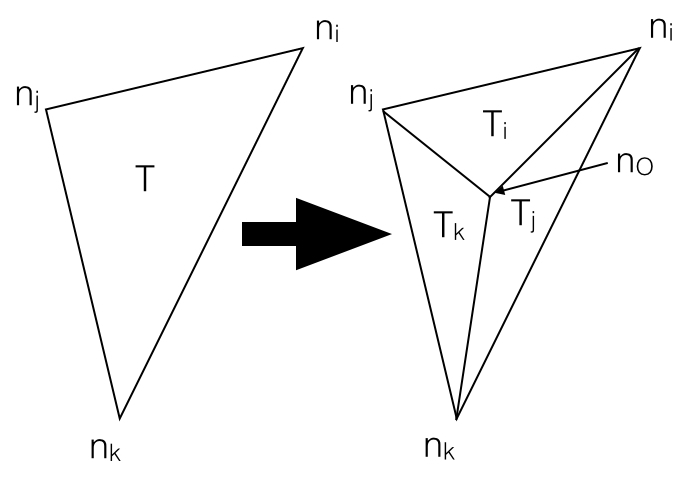
\includegraphics[height=1.4in]
    {Figures/TriangleSplit.jpg}}
  \caption{Triangle Split}
\end{figure}

The process of determining where to split a triangle is defined here by
a locally optimizing an objective function defined for a triangle: Let
$S(u,v)$ be a parameterized surface, $D$ be be a discretization of the
surface, and $T$ be a triangle (included in $D$) defined by an ordered
tuple of nodes, $\left(n_i, n_j, n_k\right)$. These nodes are ordered
such that the triangle normal is positive. Specifically, if $\vec{V_0} =
\left\{n_j - n_i \right\}$ and $\vec{V_1} = \left\{n_k - n_i\right\}$
then the triangle normal, $N_T = \vec{V_0} \times \vec{V_1}$, is
positive. Note that a two-dimensional cross-product (or two-dimensional
curl) is a scalar quantity. Additionally, let a node on the interior of
$T$ be defined as $n_O$. The four nodes, $n_i$, $n_j$, $n_k$, and $n_O$
define three triangles, $T_i\left(n_i,n_j,n_0\right), T_j\left(n_j, n_k,
n_0\right), T_k\left(n_k, n_i, n_0\right)$. If $A(T)$ is a function
that calculates the area of a triangle in $\left(x,y,z\right)$ space,
then the optimization problem for finding the optimal position for $n_0$
in $T$ is defined as:

\begin{eqnarray*}
\begin{array}{rcl}
\underset{n_O}{\text{minimize}} \ O(T) & = & - \frac{A\left(T_i\right) + A\left(T_j\right) + A\left(T_k\right) }{ A\left(T\right) }\\
\text{subject to} \ N_{T_i} & > & 0 \\
N_{T_j} & > & 0 \\ 
N_{T_k} & > & 0. \\
\end{array}
\end{eqnarray*}

It should be noted that this definition of representation deficit would
be difficult to derive or express for a topological entity other than a
triangle. This is due to the inherent ambiguity in the definition of not
only the surface area, but also the surface representation of (possibly)
non-planar elements, e.g. non-planar, or skew, quadrilateral. [MORE
POSSIBLY]

\subsection{Edge Split}
An edge in parametric space represents a (possible) curve on the
surface. Any edge, with length $L_E$, can have at most the same length
as the portion of the surface which it represents, $L_S$. Therefore, the
representation deficit for an edge, $RD_E$, is defined as $RD_E =
\frac{L_S - L_E}{L_E}$. Note that the lengths are calculated in
${\mathbb R}^3$. The difference in length, $\left(L_S - L_E\right)$, is
normalized by $L_E$ so that the result is scale independent. Also, this
is a representation {\it deficit} since $L_S \ge L_E$ is always true;

In order to apply the above definition of representation deficit to mesh
generation, a replacement for $L_S$ must be determined since the length
along the surface represented by $L_S$ is not always able to be
determined -- or, most often, the arc-length calculation is impractical.
Generally, in order to reduce the representation deficit for an edge the
edge is split by inserting an interior point. Any point that is inserted
into the interior of the edge would decrease the representation deficit
--- or at worst it will remain the same. However, the determination of
where to split the edge should be done in such a way that the
representation deficit is minimized. This strategy of refinement,
refining each edge in such a way that the representation deficit is
locally minimized, would take advantage of the optimal substructure of
the discrete topology. A method for generating a locally optimal edge
split is detailed in \cite{mclaurin12,mclaurin13}[OTHERS].

\begin{figure}[h!]
  \center{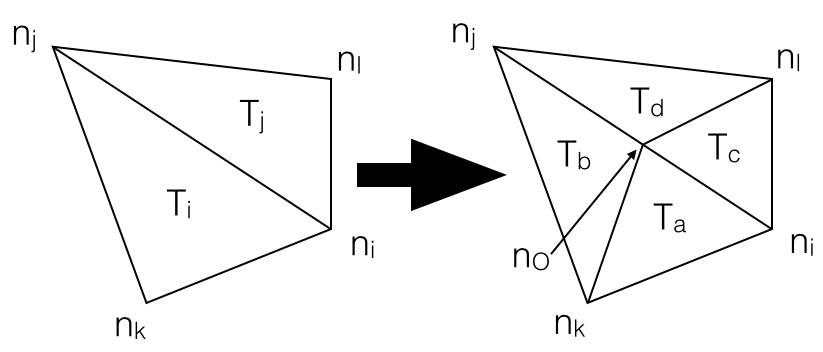
\includegraphics[height=1.4in]
    {Figures/EdgeSplit.jpg}}
  \caption{Edge Split}
\end{figure}

In addition, the fact that an edge split will change the surface area of
the discretization should be considered. Since the overall justification
of this work is reduce the {\it area} representation deficit of a
discretization, the representation deficit will not be defined for an
edge but for an edge-split. Therefore, for a given edge, only the
edge-split that minimizes {\it area} representation deficit is
considered. The process of determining where to split a triangle is
defined here by locally optimizing an objective function defined for an
edge-split.  Let $E\left(n_i,n_j\right)$ be an edge in $D$ that is
topologically adjacent to two triangles, $T_i\left(n_i,n_j,n_k\right)$,
and $T_j\left(n_i,n_l,n_j\right)$. Additionally, let a node on the
interior of the edge be defined as $n_O$. The five nodes,
$\left\{n_i,n_j,n_k,n_l,n_O\right\}$ define four triangles,
$T_a\left(n_i,n_O,n_k\right)$, $T_b\left(n_O,n_j, n_k\right)$,
$T_c\left(n_i,n_l,n_O\right)$, $T_d\left(n_O,n_l,n_j\right)$.  The
optimization problem for finding the optimal position for $n_O$ on $E$
is defined as:

\begin{eqnarray*}
\begin{array}{rcl}
\underset{n_O}{\text{minimize}} \ O(E) & = & - \frac{ A\left(T_a\right) + A\left(T_b\right) + A\left(T_c\right) + A\left(T_d\right) }{ A\left(T_i\right) + A\left(T_j\right) } \\
\text{subject to} \ N_{T_a} & > & 0 \\
N_{T_b} & > & 0 \\ 
N_{T_c} & > & 0 \\
N_{T_d} & > & 0. \\
\end{array}
\end{eqnarray*}

\subsection{Edge Swap}
Is it possible to have an optimal topology? If so, then it should be
reachable through repeated edge flipping. Therefore, we should be able
to write some sort of formulation for a pair of triangles and go from
there? [SUZANNE] Comment: for the sake of not doing any more coding, if
your ethics can let you come to the conclusion that this is either not
possible or not practical then this would fit into the
logic/justification in the next section.

% NOTE:  I suggestion we rename this subsection.  Whenever optimization is 
%   used, the term smoothing is no longer used, as smoothing can lead
%   to a decrease in the metric being measured.  With mesh quality, the 
%   appropriate term is mesh quality improvement.  I would have used the 
%   term mesh representation deficit improvement here.  However, since
%   this is a subsection and all subsection titles should be parallel,
%   that doesn't quite work either.  Can you think of a better title?

\subsection{Nodal Smoothing}
In this paper, the focus is on using nodal smoothing in 
order to locally minimize the representation deficit in the surface mesh.  
It should be noted that, although a locally optimal mesh topology could 
also be obtained, computing such a topology would involve the solution of 
a discrete optimization problem (via integer programming) which would 
specify the relevant sequence of edge flips.  The discrete 
and continuous optimization problems could then be solved in an iterative, 
interleaving fashion.  However, such an approach would require significant 
additional computational expense.

For a node, $N_i$, the representation deficit is defined only by
comparing it to the node when located at another point in space. Here
the comparison is bound by limiting the range of comparison within the
edge-hull topologically adjacent to $N_i$. Formally, let $N_i$ be a node
in $D$ that is shared topologically by $n$ triangles, where $n$ is the
face-valence of $N_i$. The optimization for finding the optimal position
for $N_i$ is defined as:

\begin{eqnarray*}
\begin{array}{rcl}
\underset{N_O}{\text{minimize}} \ O(N) & = &
-\sum{_{j=1}^{n_t-1}A\left(T_j\right)} \\
\text{subject to} \ N_{T_1} & > & 0 \\
N_{T_2} & > & 0 \\ 
N_{T_3} & > & 0 \\
& \vdots & \\
N_{T_{n-1}} & > & 0 \\ 
N_{T_n} & > & 0.
\end{array}
\end{eqnarray*}

\begin{figure}[h!]
  \center{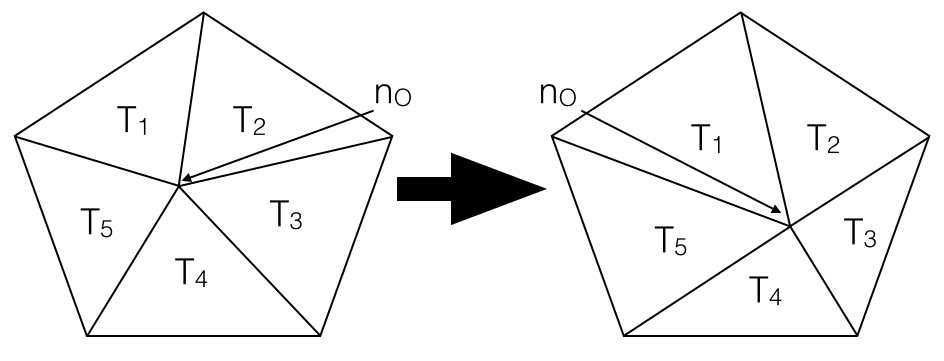
\includegraphics[height=1.4in]
    {Figures/NodalSmoothing.jpg}}
  \caption{Nodal Smoothing}
\end{figure}

[NEED TO DISCUSS HESSIAN/METRIC BASED MESH ADAPTION IN THE NODAL
SMOOTHING SECTION OF THE PAPER. THERE IS NO GLOBAL, STATIC FUNCTION
AGAINST WHICH THE INTERPOLATION ERROR CAN BE MINIMIZED. THAT IS,
WHENEVER THE MESH MOVES, THE INTERPOLATION ERROR FIELD CHANGES.]


\subsection{Boundary Refinement}
[Is there a section needed on this? It'd be straightforward to talk about
but would be pretty repetitive and I don't have it coded up yet. If I do
talk about it then due diligence says I should show some results and
there are already tons of variables to consider. This might get left out
due to space concerns.]
[This should be an argument for applying [CITE SELF] to the boundary
curves first because the interior of the surface is not what the
boundary curves are really trying to represent]


\section{Mesh Refinement Algorithm}
In order to formulate an optimization problem which, when solved, yields 
an optimal mesh triangulation based on representation deficit, a local 
optimization approach~\cite{nocedal_wright_book} is used. Such a 
formulation comes much more naturally than does a formulation based on 
global optimization~\cite{global_optimization_book} when the 
mesh operations defined in Section \ref{sec:meshoperations} are 
employed. One reason for this is the variety of mesh operations that are 
performed at different stages in the mesh generation process; they 
naturally lend themselves to the formulation of different (but related) 
optimization problems as opposed to one unified optimization problem.

It should also be noted that global optimization algorithms are typically 
not used to solve optimization problems with a large number of variables 
-- even if the problem is formulated as a global optimization problem. 
Since there are typically millions to billions of nodes and elements in 
meshes from application problems of interest, a global optimization 
problem would be impractical solve based on the huge number of variables 
that it would necessarily contain. In addition, any global optimization 
problem which would be formulated as a generalization of the local 
optimization problems in this work would be a continuous optimization 
problem. Typically global optimization methods are designed for use on 
discrete optimization problems or on contious optimization problems with 
convex objective functions with guaranteed global minima.

For the above reasons, iterative refinement (a local optimization 
approach) is used to find optimal substructures at each stage of the mesh 
generation process. The local optimization technique employed is
motivated by a class of optimization methods called pattern search 
techniques~\cite{patternsearch1}. Pattern search and multidirectional 
search techniques were developed by Park and Shontz for mesh quality 
improvement~\cite{patternsearch4}; their techniques were based on the 
underlying classes of optimization methods in the literature. Pattern 
search methods do not use derivatives and hence can be used on problems for 
the most general problems for which derivatives either do not exist or are 
impractical to compute.

The optimization employed here uses a simple ``cross'' pattern (up down
left right center, \cite{crossPattern}) {\bf{Dave:  No reference by
with this label appears in the References currently.  Please 
update}} which 
is sized based on the
local geometry so that it could be moved inside of the triangles/hulls
many times before encountering the boundary. In the case of triangle
splitting, the cross was sized as $0.001$ multiplied by the average edge
length of the triangle. In the case of node movement, the cross was
sized as $0.001$ multiplied by the average edge length of the
topologically attached edges. The cross pattern was not resized during
optimization.  Additionally, the search was not allowed to create
inverted elements.  This was enforced by halting a search whose next
step would create any overlapping edges, tangled elements, etc... Care
was taken to ensure that convergence of the local optimization method
was obtained; this is important since criteria must be met in order for
the heuristic pattern search methods to
converge~\cite{patternsearch2,patternsearch3}.

\begin{figure}
  \begin{center}
  \label{crossPattern}
  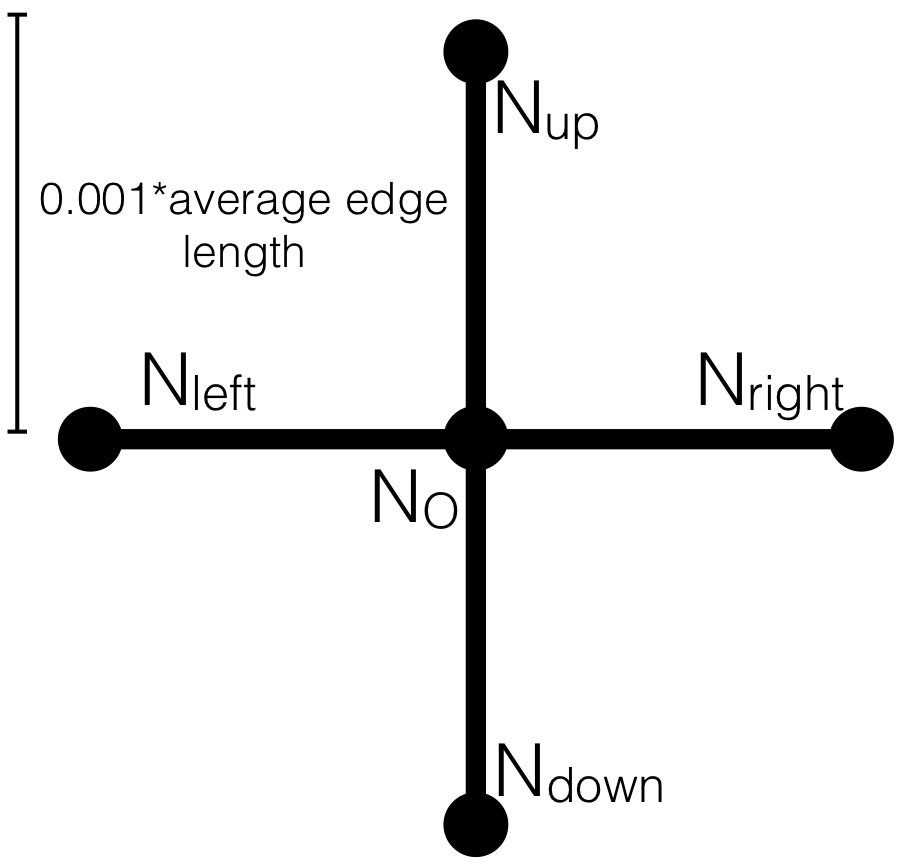
\includegraphics[width=50mm]{Figures/crossPattern.png}
  \caption{Cross Pattern used for Pattern Search Optimization}
  \end{center}
\end{figure}


The following algorithm is used to generate an optimal triangulation
based on representation deficit refinement:

\subsection{Algorithm Specification}
\begin{algorithm}[H]
\begin{algorithmic}
\caption{Find optimal point for triangle splitting}
\Procedure{findOptimalPoint}{$t_i$} \Comment{for Triangle}
  \State $pattern \gets sizePattern\left( t_i \right)$
  \State $pattern \gets calculateTrianglePatternValues\left( t_i \right)$
  \State $minValue \gets determineMinPatternValue\left( pattern \right)$
  \While{$newTriangulationIsValid\left( minValue \right)$}
    \State $pattern \gets shiftPattern\left( minValue \right)$
    \State $pattern \gets calculateTrianglePatternValues\left( t_i \right)$
    \State $minValue \gets determineMinPatternValue\left( pattern \right)$
  \EndWhile
  \State $p_i \gets currentPatternValue\left( pattern \right)$
  \State $return \gets \left( p_i, minValue \right)$
\EndProcedure
\end{algorithmic}
\end{algorithm}

\begin{algorithm}[H]
\begin{algorithmic}
\caption{Find optimal point for edge splitting}
\Procedure{findOptimalPoint}{$e_i$} \Comment{for Edge}
  \State $pattern \gets sizePattern\left( e_i \right)$
  \State $pattern \gets calculateEdgePatternValues\left( e_i \right)$
  \State $minValue \gets determineMinPatternValue\left( pattern \right)$
  \While{$newTriangulationIsValid\left( minValue \right)$}
    \State $pattern \gets shiftPattern\left( minValue \right)$
    \State $pattern \gets calculateEdgePatternValues\left( e_i \right)$
    \State $minValue \gets determineMinPatternValue\left( pattern \right)$
  \EndWhile
  \State $p_i \gets currentPatternValue\left( pattern \right)$
  \State $return \gets \left( p_i, minValue \right)$
\EndProcedure
\end{algorithmic}
\end{algorithm}

\begin{algorithm}[H]
\caption{Iterative Refinement}
\label{alg_IterativeRefinement}
\begin{algorithmic}
\Procedure{TriangleRefine}{$T$, $tol_{RD}$} \Comment{Refine the triangulation, $T$}
  \For{each triangle, $t_i$}
    \State $\left( p_i, minValue \right) \gets findOptimalPoint\left( t_i \right)$
    \If{$tooCloseToEdge\left( p_i, t_i \right)$}
      \State $e_i \gets findNearEdge\left( p_i, t_i \right)$
      \State $\left( p_i, minValue \right) \gets findOptimalPoint\left( e_i \right)$
      \State $operation \gets EdgeSplit\left( e_i, p_i \right)$
    \Else
      \State $operation \gets triangleSplit\left( t_i, p_i \right)$
    \EndIf
    \If{$minValue < tol_{RD}$}
      \State perform $operation$
    \EndIf
  \EndFor
\EndProcedure
\end{algorithmic}
\end{algorithm}

\begin{algorithm}
\begin{algorithmic}
\caption{Find the optimal point for node relocation}
\label{alg_NodeSmoothing}
\Procedure{findOptimalPoint}{$n_i$} \Comment{for Node}
  \State $pattern \gets sizePattern\left( n_i \right)$
  \State $pattern \gets calculateNodePatternValues\left( n_i \right)$
  \State $minValue \gets determineMinPatternValue\left( pattern \right)$
  \While{$newTriangulationIsValid\left( minValue \right)$}
    \State $pattern \gets shiftPattern\left( minValue \right)$
    \State $pattern \gets calculateNodePatternValues\left( n_i \right)$
    \State $minValue \gets determineMinPatternValue\left( pattern \right)$
  \EndWhile
  \State $p_i \gets currentPatternValue\left( pattern \right)$
  \State $return \gets \left( p_i, minValue \right)$
\EndProcedure
\end{algorithmic}
\end{algorithm}

\begin{algorithm}[H]
\caption{Nodal Movement}
\begin{algorithmic}
\Procedure{NodalSmooth}{$T$, $tol_{RD}$} \Comment{Smooth Node Positions}
  \For{each node, $n_i$}
    \State $pattern \gets sizePattern\left( e_i \right)$
    \State $pattern \gets calculateNodePatternValues\left( n_i \right)$
    \State $\left( p_i, minValue \right) \gets findOptimalPoint\left( e_i \right)$
  \EndFor
  \If{$minValue < tol_{RD}$}
    \State relocate $n_i$ to $p_i$
  \EndIf
\EndProcedure
\end{algorithmic}
\end{algorithm}

\subsection{Observations}
\subsubsection{Nodal Movement}
In practice, it was observed that nodes will often move toward each other
when there is a ``local minimum'' nearby ({\it race-condition}).
However, once the two nodes get sufficiently near to each other, one will
inevitably get nearer to the local minimum first and the other node will
be ``pushed'' away.

\subsubsection{Edge Flipping}
Another phenomenon that was noticed was that during triangle splitting
and node movement, a node would often be repositioned near edges. This
usually meant that the nearby local minimum was either on the edge or on 
the other topological side of the edge. Without some sort of intervention,
this would lead to nearly degenerate geometry being formed. In order to
prevent geometry which could cause numerical robustness issues, when a
node neared an edge during node movement the edge was flipped. This
allowed the node to move unobstructed by the newly-reconnected edge.

The criteria for determining if a node is ``too close'' to an edge is
based on the size of the pattern. Once the node gets within $1\%$ of the
average edge length, which equates to $10$ times the pattern size, it is
considered ``too close''. There is a balance here between preventing the
creation of degenerate geometry and allowing the pattern search to find
{\it and then use} an optimum value. The above heuristics were found to
be a good compromise and will be shown to be effective. If the minimum
value for the objective function is on or across an edge, then the edge
is flipped and the process is repeated with the new topology.



\section{Results}
In this explorative work, results will be shown for the how each
individual mesh operations (triangle split, edge split, node movement)
affects the representation deficit. In addition, an effective
combination of the aforementioned mesh operations was developed and the
results will be shown. The geometry which is being discretized is the
``peaks'' function which has a well-known parametrization
\cite{peaksMatlab}. The domain was chosen so that the boundary is
sufficiently far away from the local minima/maxima present near the origin to
show that the developed scheme is efficient at reducing representation
deficit. The $x$ and $y$ values are each confined between $-5.0$ and
$5.0$ and the initial triangulation is two triangles that fill the
quadrilateral defined by the four corner points.

The main driver of representation deficit, $RD$, based mesh refinement
is the value for representation deficit. This is a ratio of the
``before'' area to the ``after'' area for each mesh operation. The
surface area of the peaks function in the given domain was calculated by
uniformly triangulating the surface with a very fine resolution. The
result was found to converge to $177.944$ with a $u$ and $v$ resolution
of 301 points. For ease of presentation, the peaks functions is shown as
a contour plot where red represents local maxima and blue represents
local minima/maxima.

\subsection{Triangle and Edge Splitting}
Restricting the mesh refinement to only triangle splits or only edges
splits is not useful, as discussed above. Therefore, the combination of
the two was performed (as described in \ref{alg_IterativeRefinement})
to produce the following results. The following figure shows the results
from $tol_{RD}=\left(0.5,0.25,0.125\right)$ from left to right. The mesh was
refined by splitting triangles and edges where appropriate as described
above.

\begin{figure}[h!]
  \begin{center}

  \subfloat[$tol_{RD}=0.5$]{\label{fig_RefineOnlyA}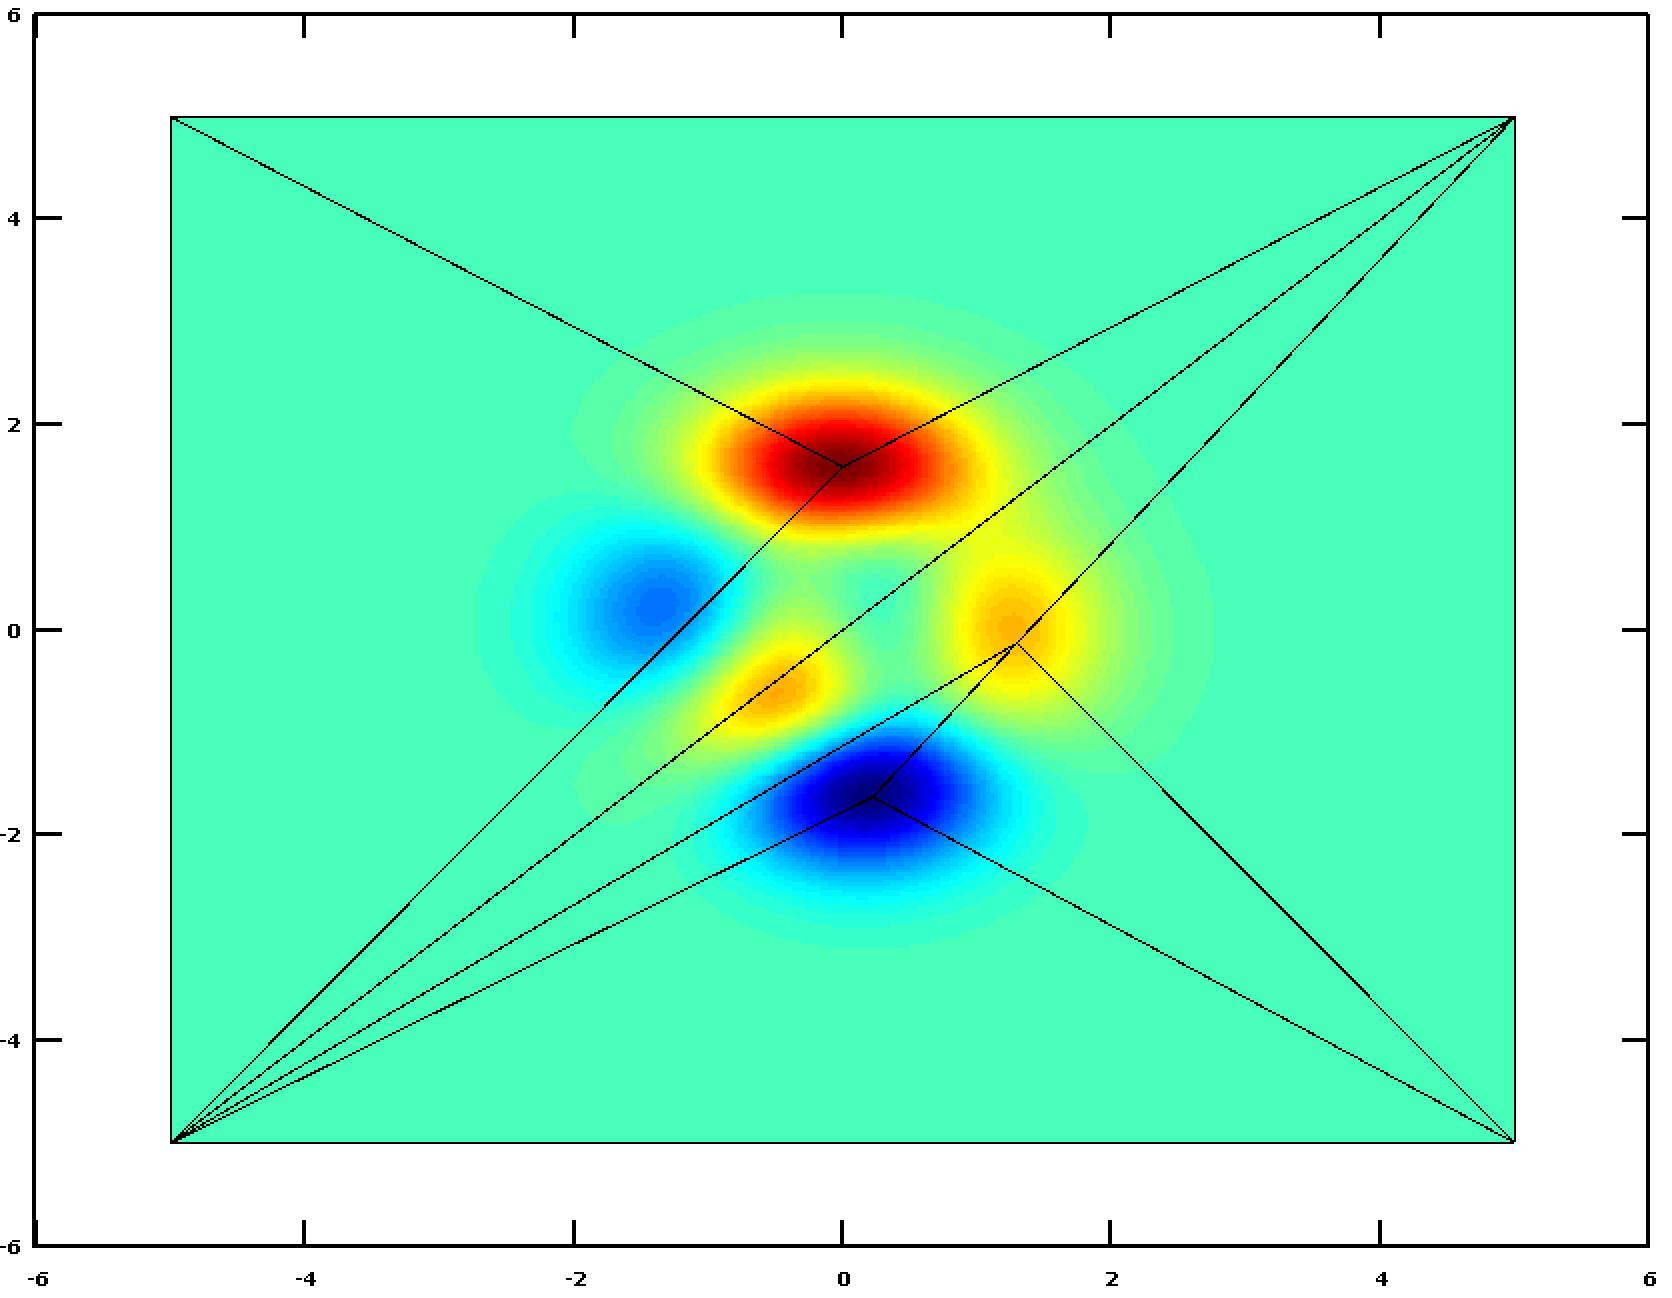
\includegraphics[width=50mm]{Figures/RefineOnly05.png}}
  \subfloat[$tol_{RD}=0.25$]{\label{fig_RefineOnlyB}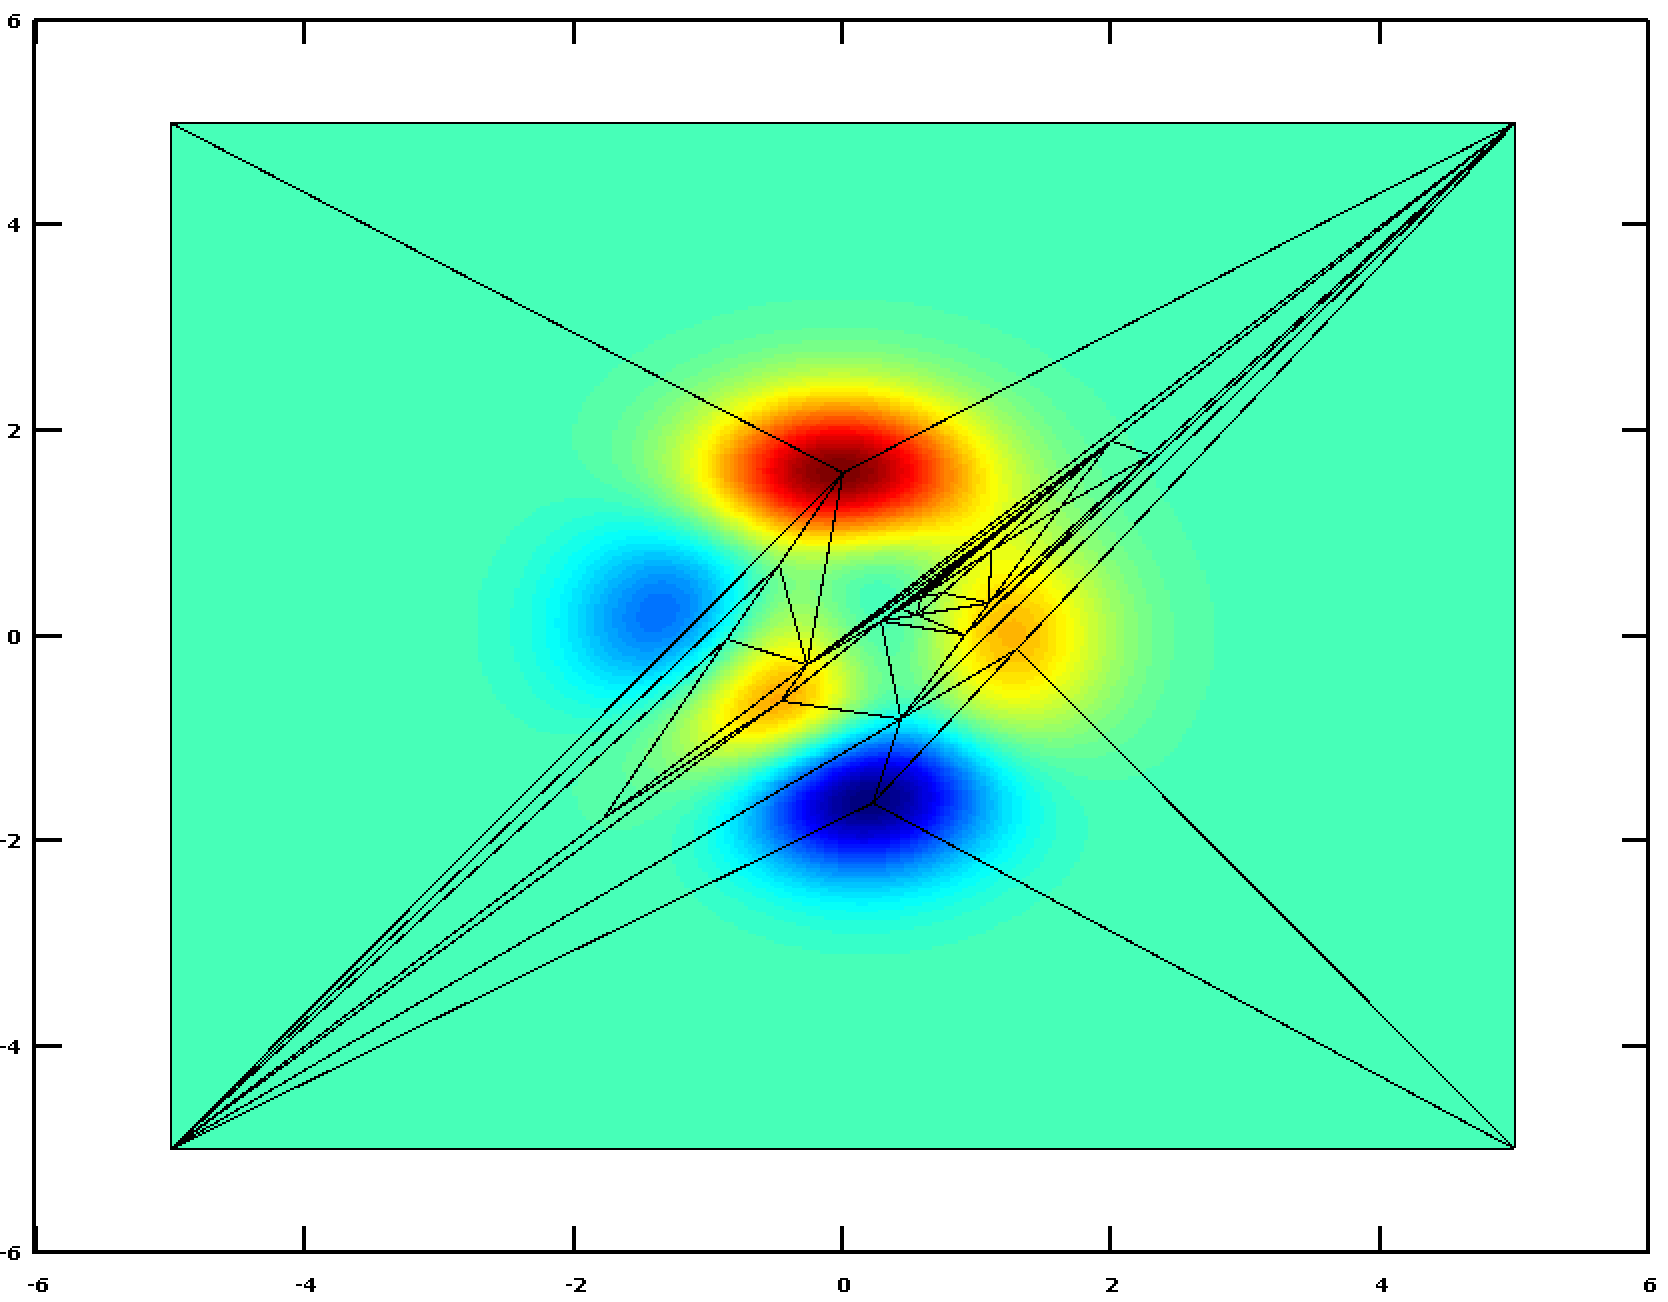
\includegraphics[width=50mm]{Figures/RefineOnly025.png}}
  \subfloat[$tol_{RD}=0.125$]{\label{fig_RefineOnlyC}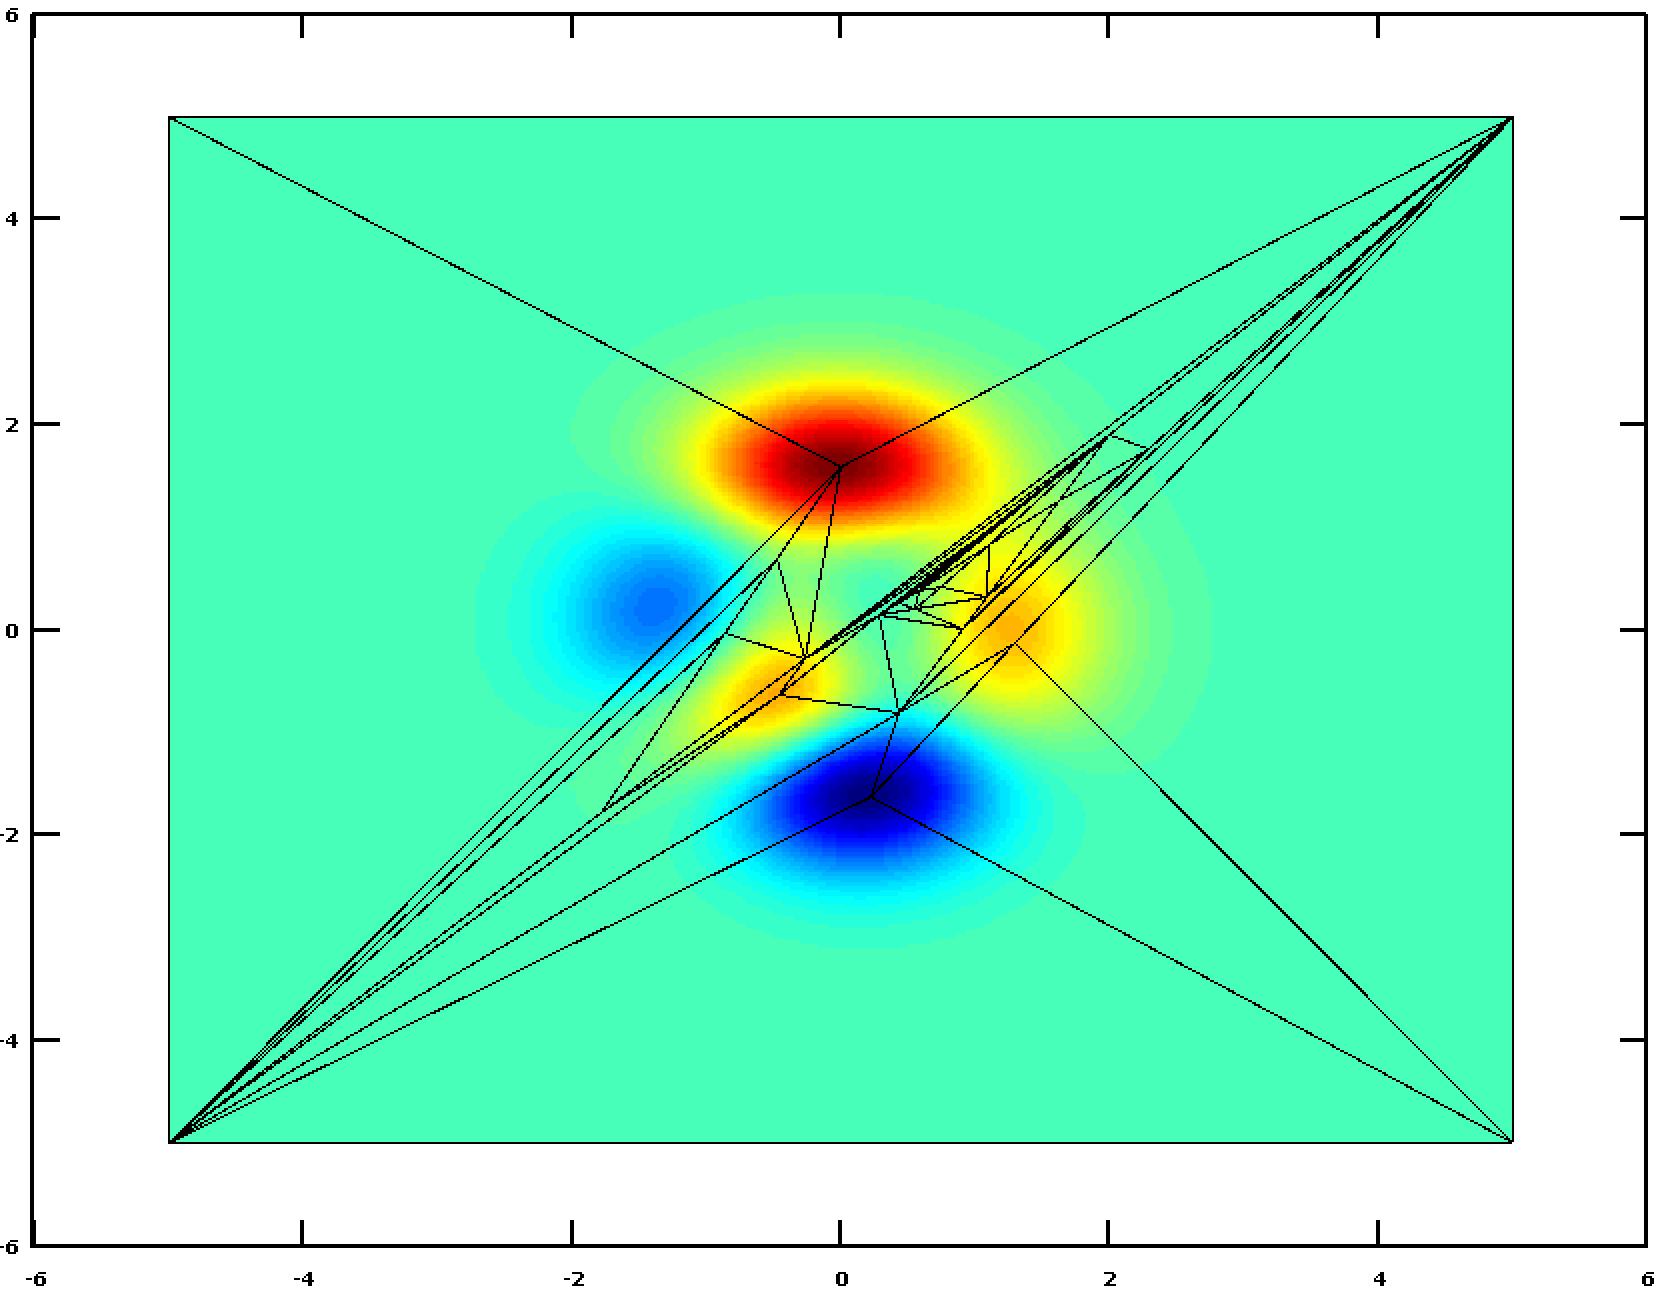
\includegraphics[width=50mm]{Figures/RefineOnly0125.png}}

  \caption{Mesh Refinement Only}
  \label{fig_RefineOnly}
  \end{center}
\end{figure}

In \ref{fig_RefineOnlyA} it can be seen that only three nodes were
inserted. This is due to the very high value of $tol_{RD}$ for this
example.  However, the nodes that were inserted were inserted very near
to the local minima/maxima of the function. If $tol_{RD}$ were halved to
$0.25$, \ref{fig_RefineOnlyB} then $92$ nodes are inserted. Again, the
nodes are inserted very near to local minima/maxima and additionally
near saddle points. If $tol_{RD}$ is halved again to $0.125$,
\ref{fig_RefineOnlyC}, no more nodes are inserted. This is due to the
very poor quality triangles.  The sliver triangles that can be seen in
\ref{fig_RefineOnlyB}, \ref{fig_RefineOnlyC} represent nearly planar section
of the mesh and therefore not refined further. This is the major
shortcoming of the developed algorithm: element quality is not
considered and this limitation leads to poor quality meshes that cannot
be refined further.

\subsection{Node Movement Effect}
In order to show the effect of node movement, the resultant mesh shown
in \ref{fig_RefineOnlyB} is used as input and the same value for
$tol_{RD} = 0.25$ is used with \ref{alg_NodeSmoothing}.

\begin{figure}[h!]
  \begin{center}
 
  \subfloat[$tol_{RD}=0.25$]{\label{fig_NodeSmoothingA}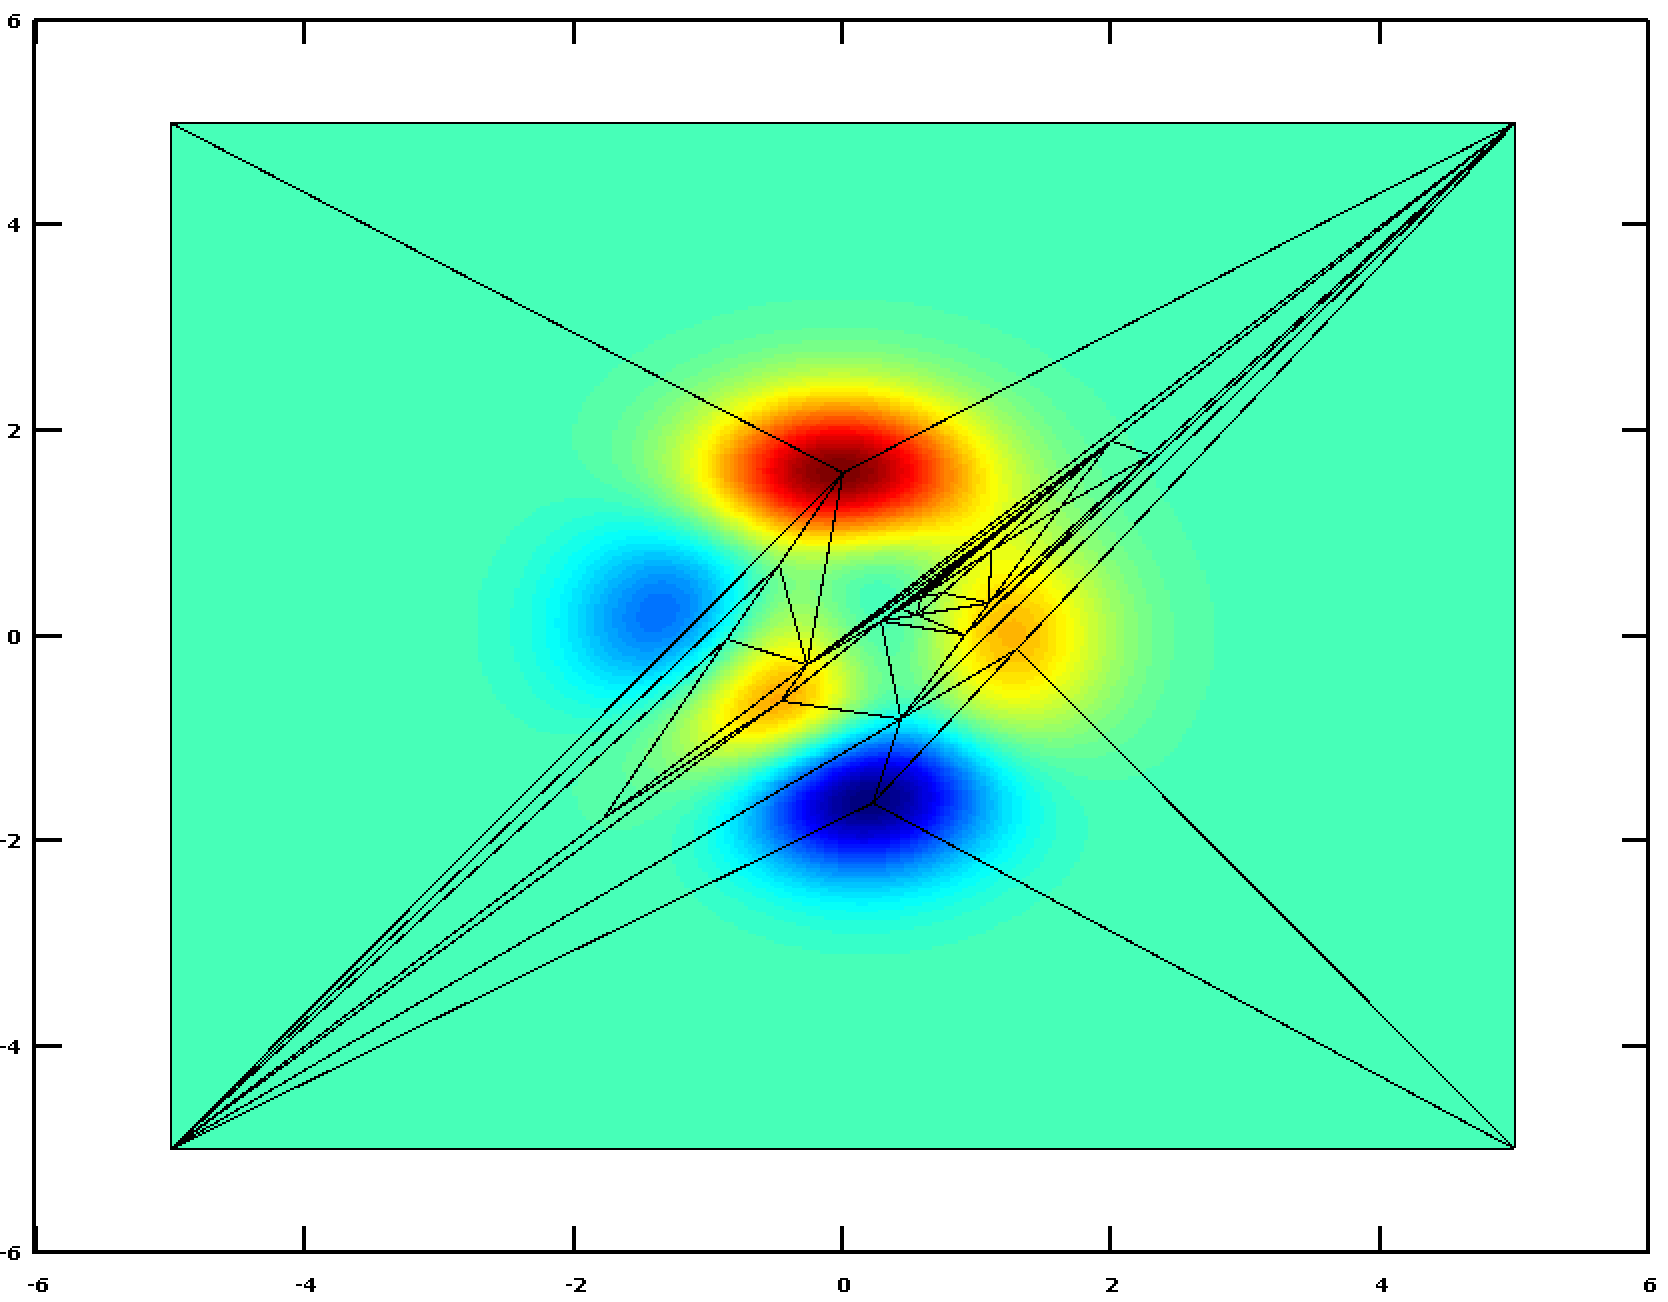
\includegraphics[width=60mm]{Figures/RefineOnly025.png}}
  \subfloat[$tol_{RD}=0.25$]{\label{fig_NodeSmoothingB}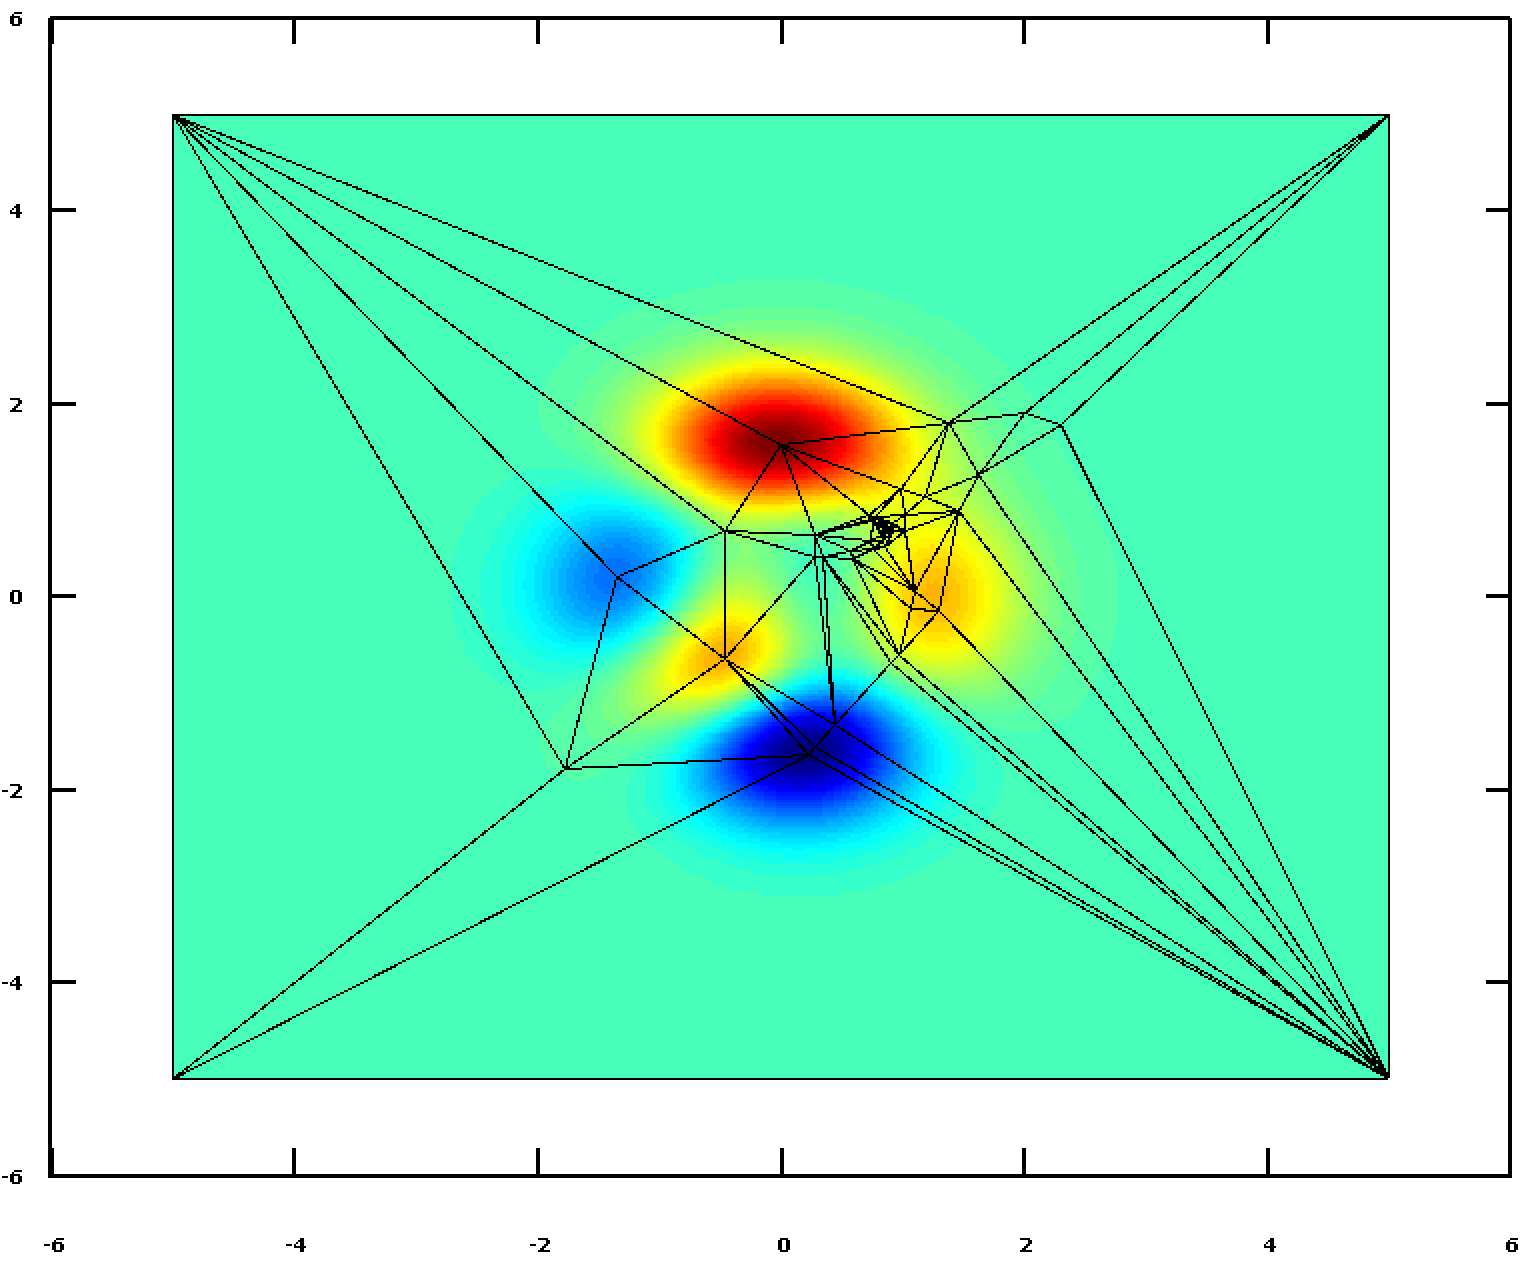
\includegraphics[width=60mm]{Figures/NodeSmooth025.png}}
  \caption{Effect of Node Movement on RD and Mesh Quality}
  \label{fig_NodeSmoothing}

  \end{center}
\end{figure}

The node movement was very effective at reducing representation deficit.
For this particular case, it reduced the representation deficit of the
input mesh by $23.36\%$. It should also be noted that the local
minima/maxima were accurately maintained by this procedure. It can also
be seen that moved nodes that were nearby but not in local minima/maxim
were moved to the local minima/maxima. Additionally, since the node
movement was allowed to perform local reconnections where needed
(discussed above), the element quality was also improved as a
side-effect.

\subsection{Effective Combination}
It easily noted that while the aforementioned mesh operations are
effective at reducing representation deficit they do not create high
quality triangles.  However, with the addition of a simple min-max edge
flip pass in between refinement and node movement passes the element
quality and representation deficit can be improved significantly.

\begin{figure}[h!]
  \begin{center}
  \subfloat[$tol_{RD}=0.25$, no movement]{\label{fig_ComboA}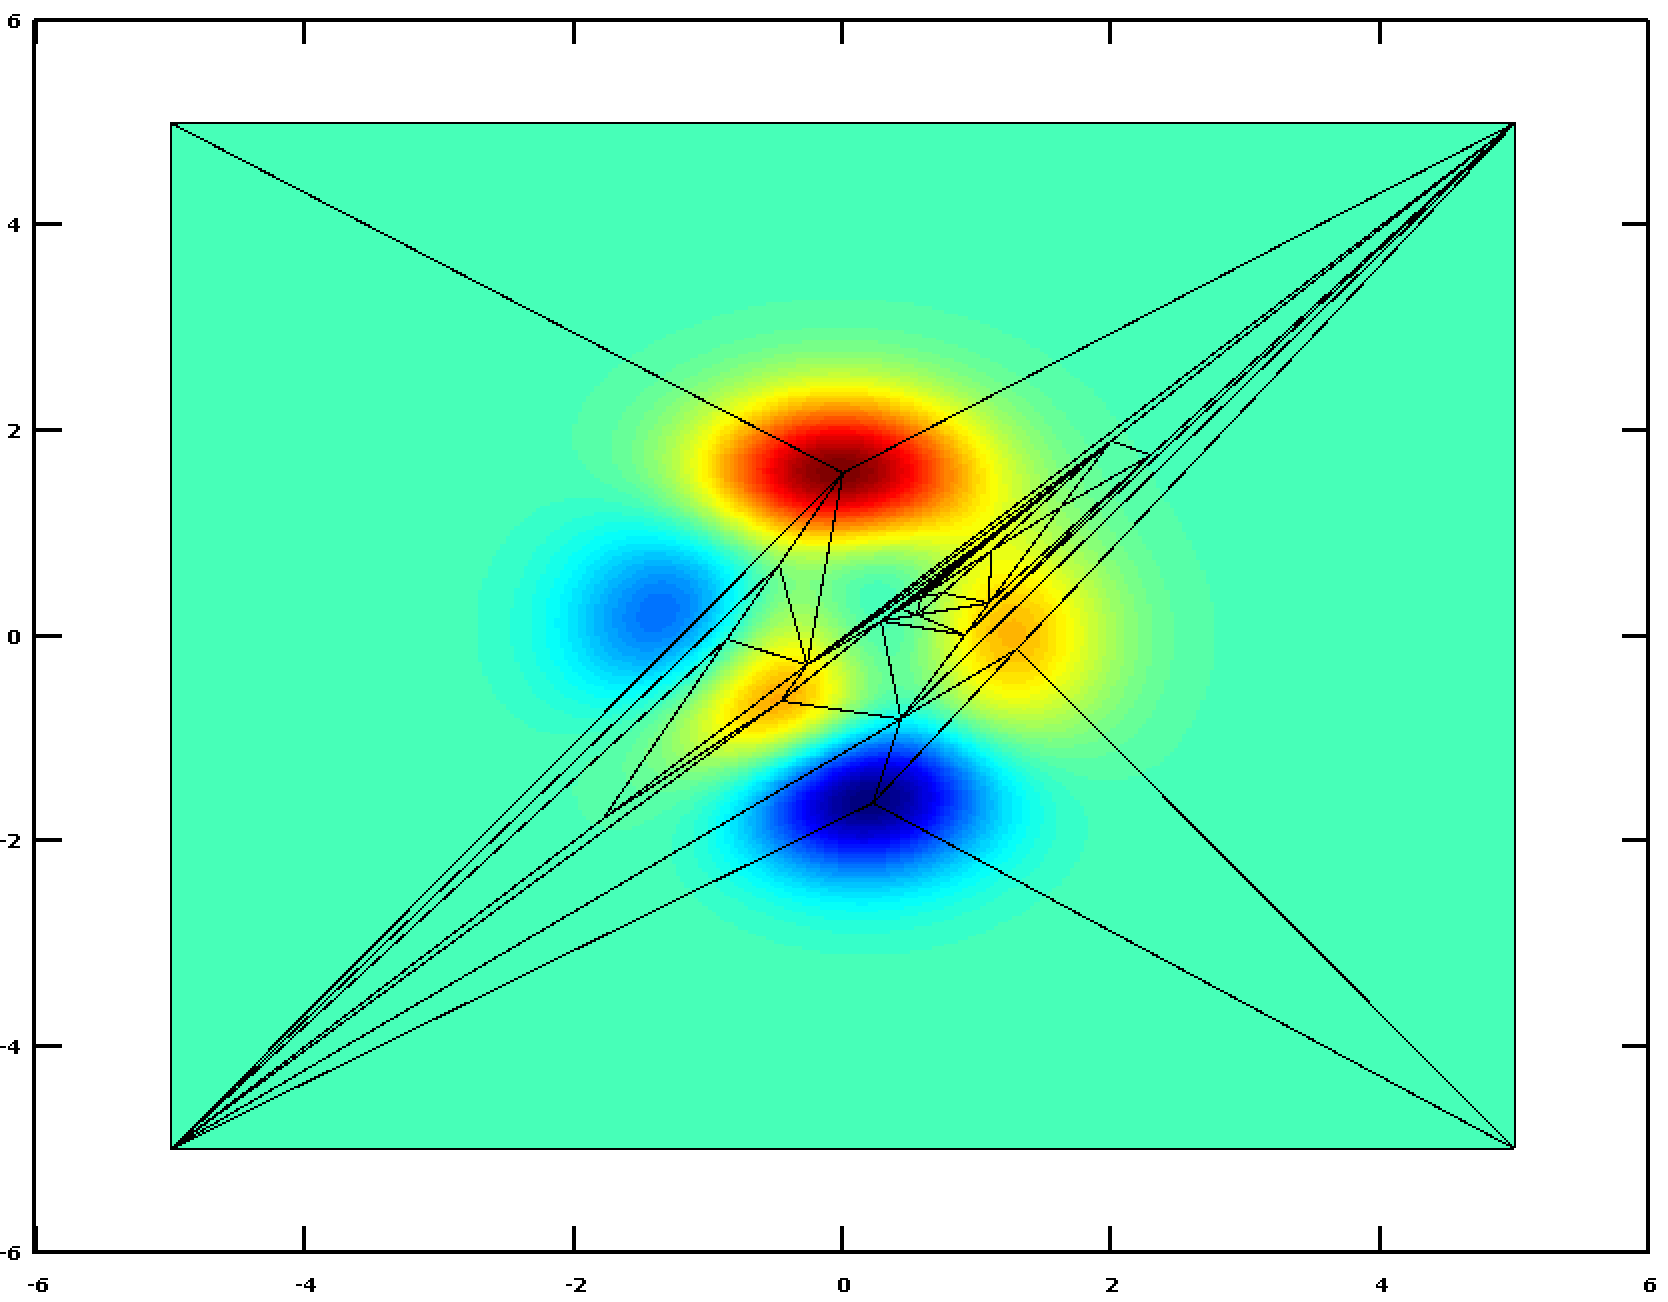
\includegraphics[width=50mm]{Figures/RefineOnly025.png}}
  \subfloat[$tol_{RD}=0.25$, movement post]{\label{fig_ComboB}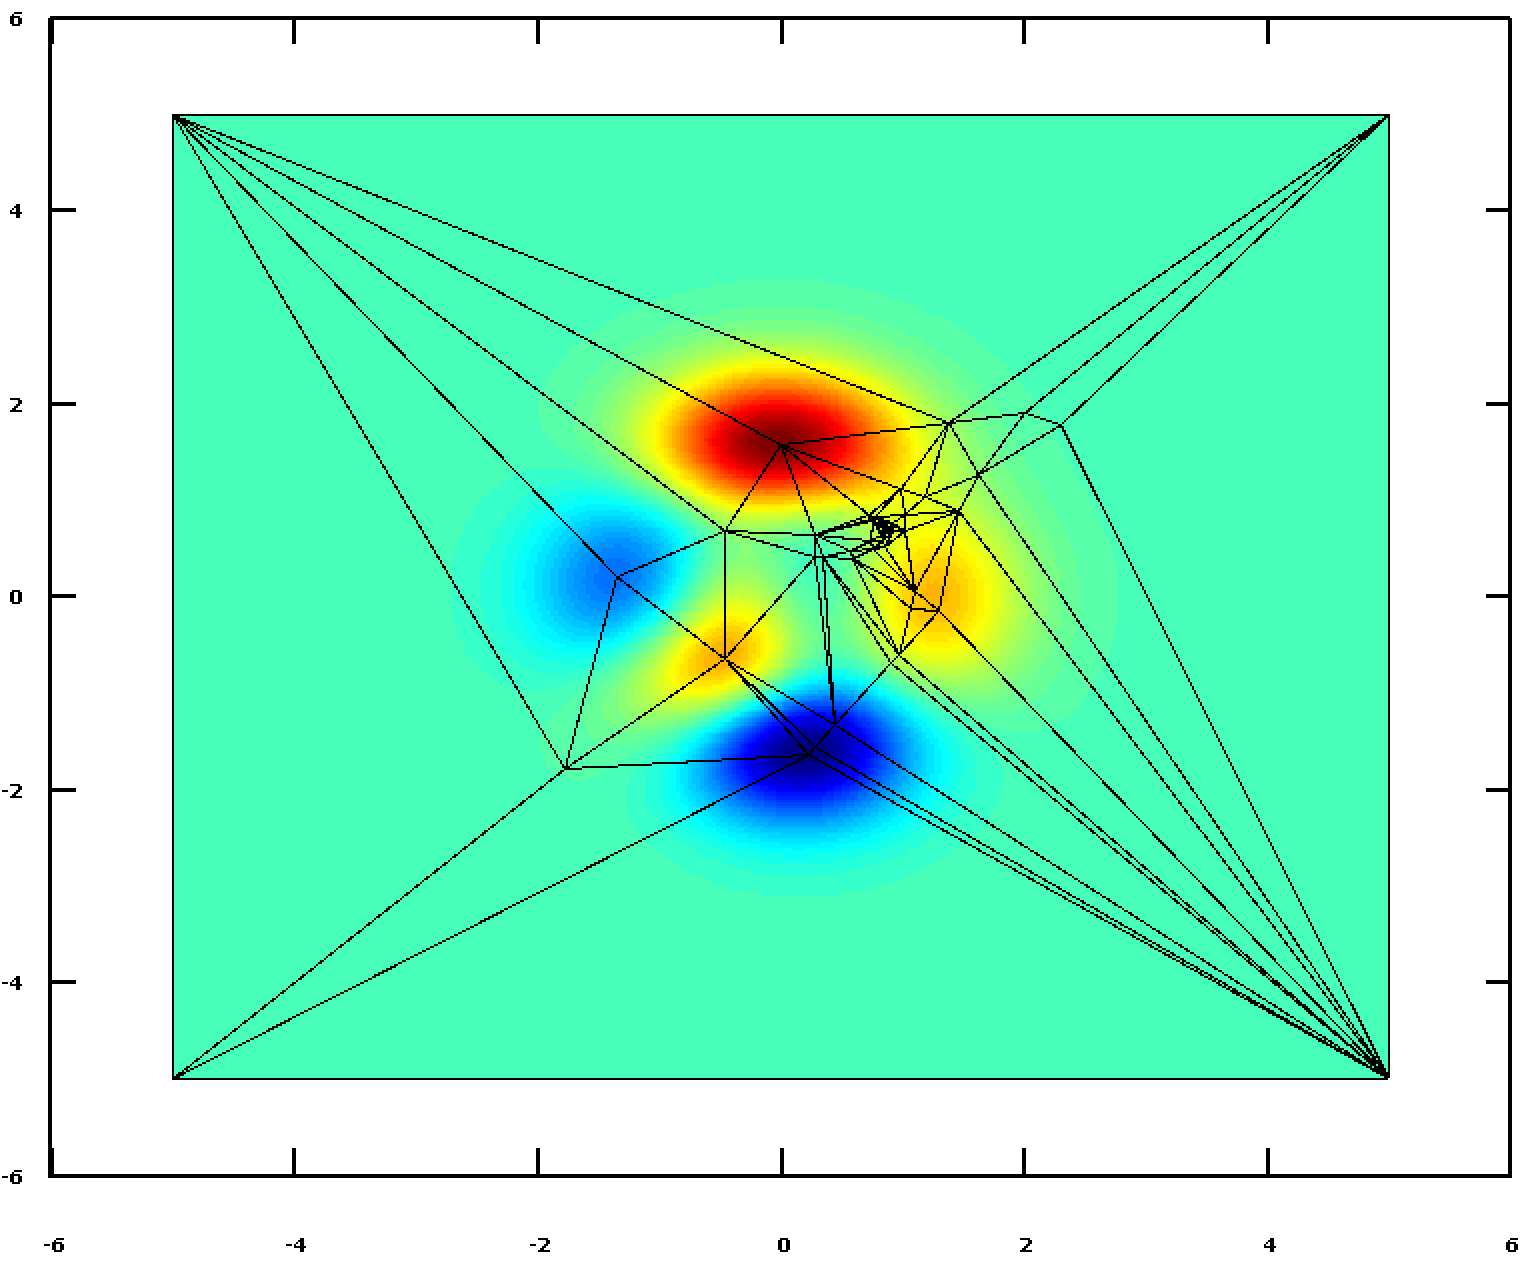
\includegraphics[width=50mm]{Figures/NodeSmooth025.png}}
  \subfloat[$tol_{RD}=0.25$, reconnection]{\label{fig_ComboC}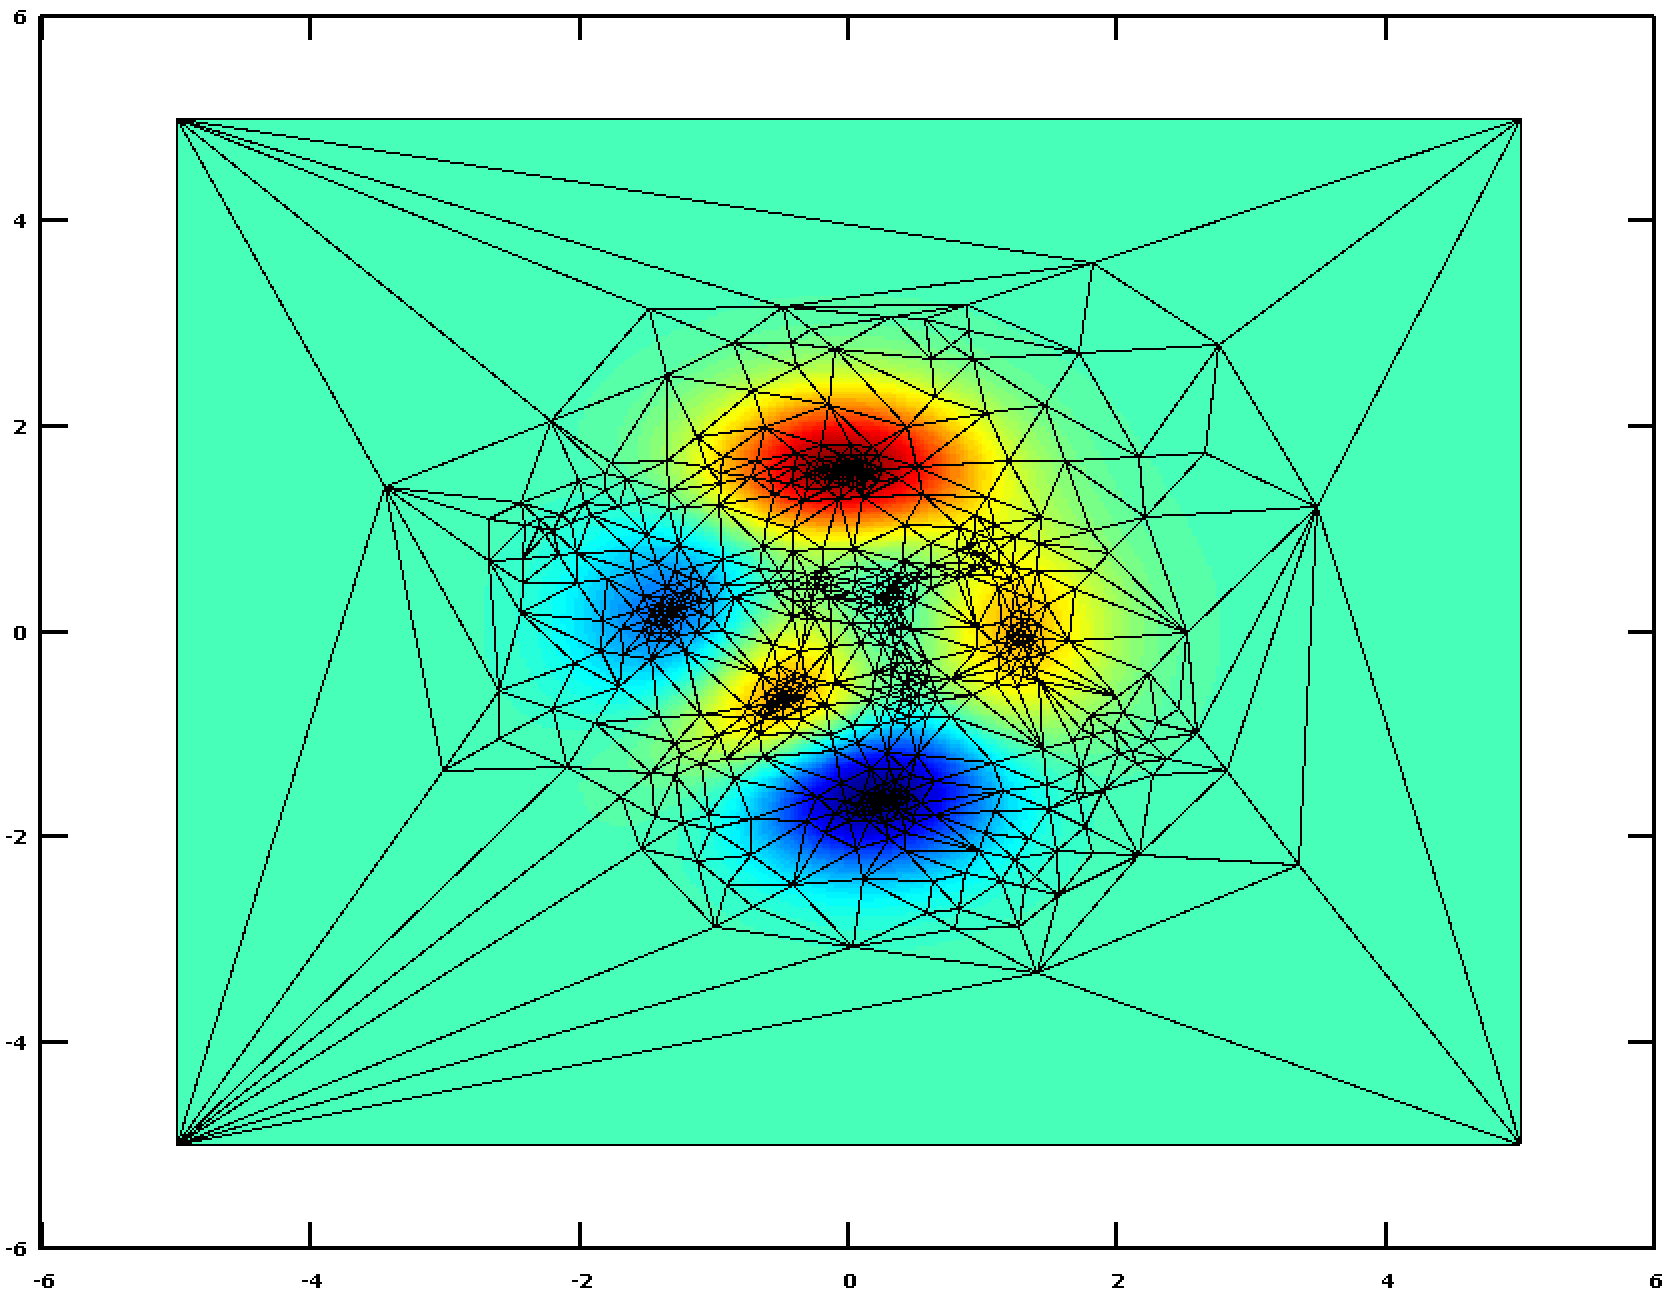
\includegraphics[width=50mm]{Figures/Reconnect025.png}}
  \caption{Comparison of Exclusive Splitting, with addition of Node
Movement, with further addition of local reconnection}
  \label{fig_NodeSmoothing}
  \end{center}
\end{figure}

In \ref{fig_ComboC} the marked difference in mesh quality and mesh
density caused by local reconnection can be seen. The addition of the
local reconnection enabled the quality of triangle to be improved every
step therefore allowed more nodes to be inserted. In this case, instead
of $92$ nodes being inserted (\ref{fig_ComboA}), $713$ nodes were
inserted. The surface area of the final mesh was $179.234$. This is a
representation deficit of $0.725\%$.

\begin{figure}[h!]
  \begin{center}
  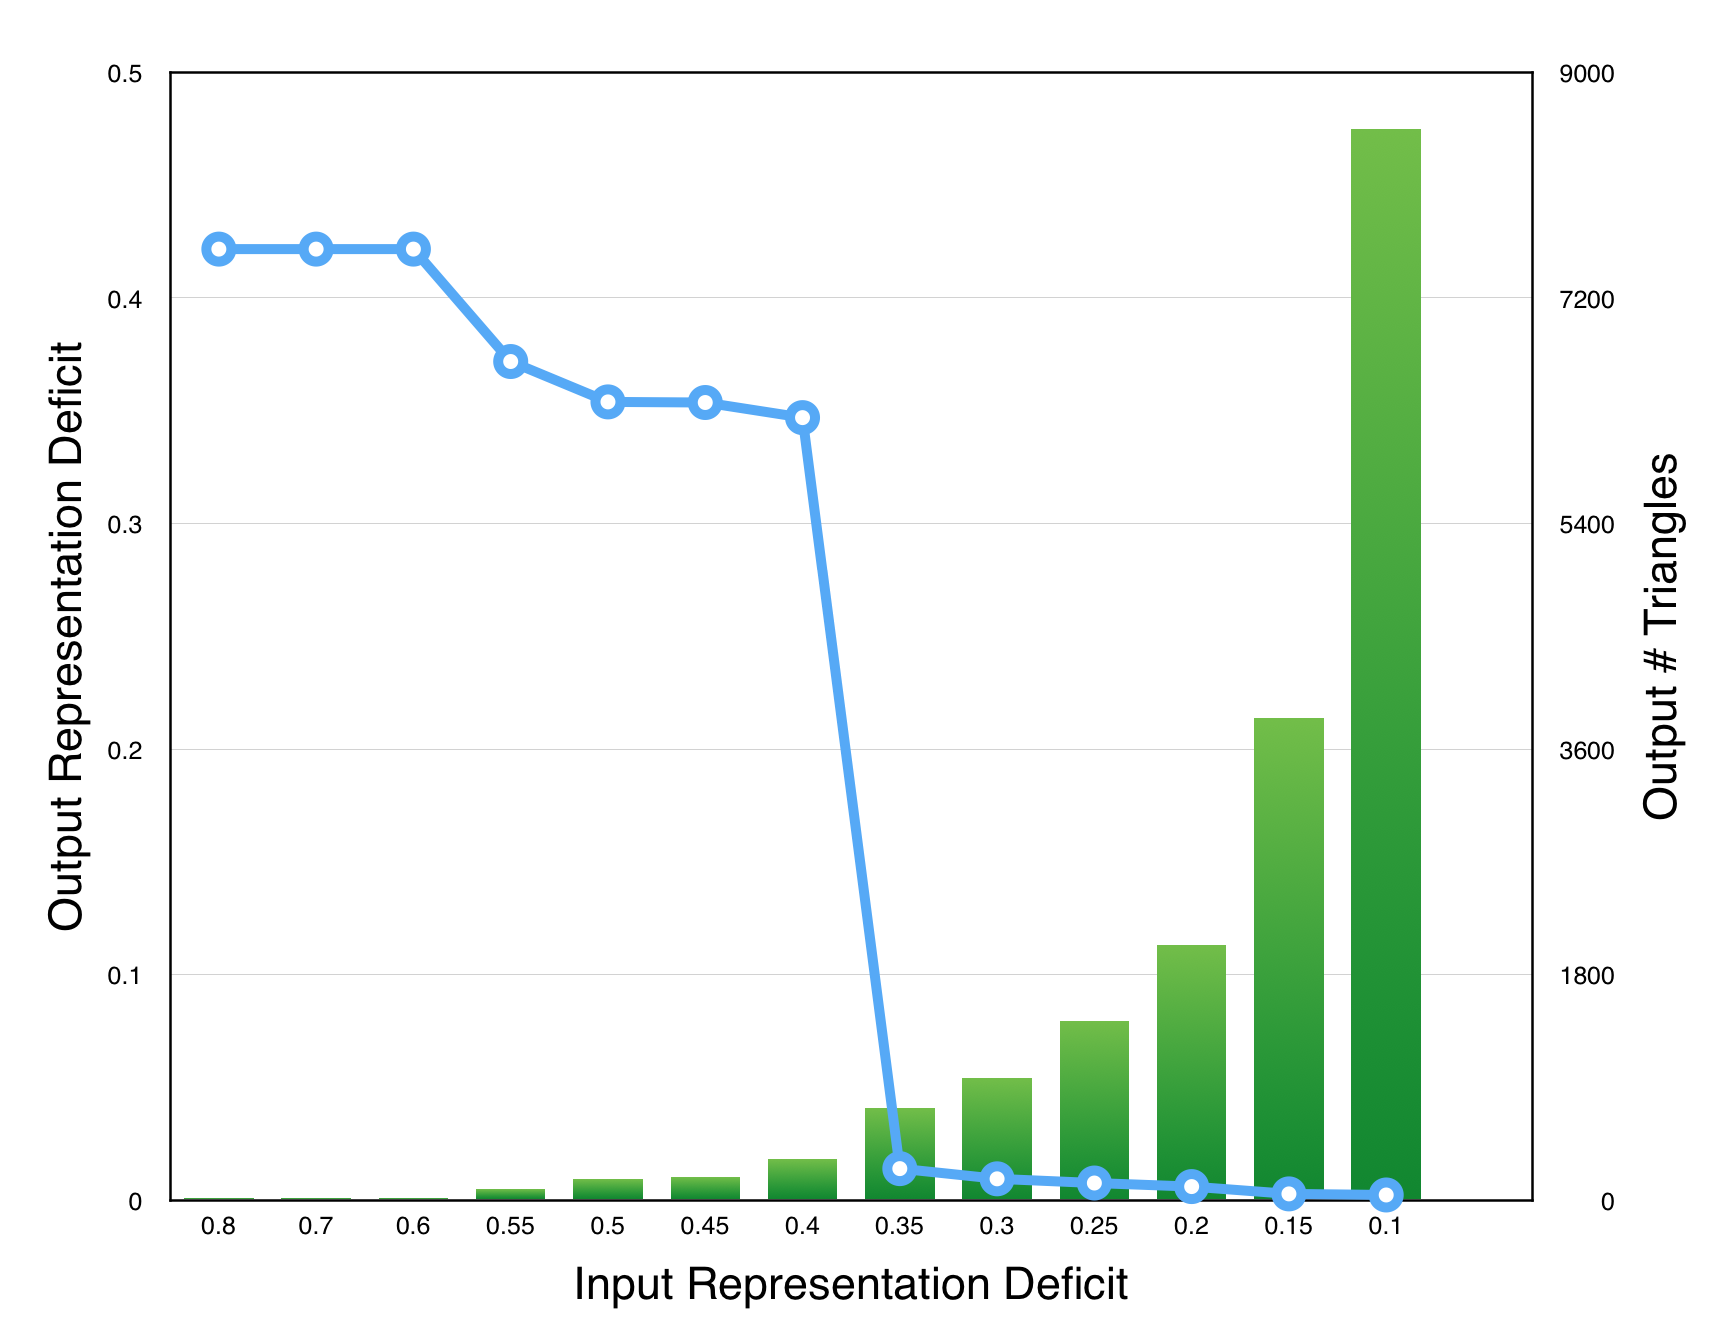
\includegraphics[width=90mm]{Figures/RDvsMeshSize.png}
  \caption{Output Surface $RD$ and Mesh Size vs. $tol_{RD}$}
  \label{fig_RDvsMeshSize}
  \end{center}
\end{figure}

A clear trend can be seen in \ref{fig_RDvsMeshSize} where as the value
of $tol_{RD}$ is decreased the representation deficit of the generated
mesh also decreases (blue line). Also, as with many optimization
problems, this particular geomtry (``peaks'' surface) and this
particular initial mesh (two triangles) have noticeable local minima in
the search space. \ref{fig_RDvsMeshSize} clearly shows three plateaus of
representation deficit in the output mesh with decreasing $tol_{RD}$.
The green bars depict the output mesh size and also convey the
diminishing returns of decreasing $tol_{RD}$ too much. Only $18$
triangles are needed for the output RD to reach $0.42$ ($42\%$).
However, an additional $156$ triangles were needed to reduce the output
RD by ten points ($\sim 35\%$). To get much nearer another local
minimum (possibly the global minimum) required many more triangles,
$738$ in total to reach $\sim 1\%$ output RD. In each case, the
optimal substructure of the problem is apparent with the value of the
value of $tol_{RD}$ being greater than the representation deficit of
the generated mesh.



\section{Conclusions}
In this work, the concept of optimal mesh refinement was explored. This
was done through the development of a formal definition for three
fundamental mesh operations, triangle split, edge split, and node
movement; each with respect to the concept of {\it representation
deficit}. Results were given showing this methodology to be an effective
method for mesh refinement. The most effective method was found to be a
combination of the above three fundamental mesh operations and delaunay
local reconnection. The representation is also efficient in that the
interior of the domain was not overly refined in order to achieve the
desired surface representation.

\subsection{Future Work}
There are several possible directions for future work.  One avenue for
future work is to further improve the optimization algorithm in the
following two ways.  First, optimization could be employed in the
determination of which mesh operation to perform at each stage of the
optimization procedure.  Second, the objective function could be
modified in order to generate surface meshes that simultaneously
minimize the representation deficit and optimize the mesh quality.
Another possibility for future research would be to extend the surface
mesh generation algorithm to handle the volume mesh generation case so
that a hierarchical approach for mesh generation (i.e., edge
grid~\cite{mclaurin13} $\mapsto$ surface mesh~\cite{mclaurin14}
$\mapsto$ volume mesh) could be employed. This would allow for
optimization of each stage of the mesh generation procedure.  Finally,
parallelization of the algorithm would allow for optimal generation of
very large surface meshes such as those required by {\bf{Dave:  Cite a
``killer'' engineering application here.}} applications.


\iffalse
% For one-column wide figures use
\begin{figure}
% Use the relevant command to insert your figure file.
% For example, with the graphicx package use
  \includegraphics{example.eps}
% figure caption is below the figure
\caption{Please write your figure caption here}
\label{fig:1}       % Give a unique label
\end{figure}
%
% For two-column wide figures use
\begin{figure*}
% Use the relevant command to insert your figure file.
% For example, with the graphicx package use
  \includegraphics[width=0.75\textwidth]{example.eps}
% figure caption is below the figure
\caption{Please write your figure caption here}
\label{fig:2}       % Give a unique label
\end{figure*}
%
% For tables use
\begin{table}
% table caption is above the table
\caption{Please write your table caption here}
\label{tab:1}       % Give a unique label
% For LaTeX tables use
\begin{tabular}{lll}
\hline\noalign{\smallskip}
first & second & third  \\
\noalign{\smallskip}\hline\noalign{\smallskip}
number & number & number \\
number & number & number \\
\noalign{\smallskip}\hline
\end{tabular}
\end{table}
\fi

%\begin{acknowledgements}
%If you'd like to thank anyone, place your comments here
%and remove the percent signs.
%\end{acknowledgements}

% BibTeX users please use one of
%\bibliographystyle{spbasic}      % basic style, author-year citations
\bibliographystyle{spmpsci}      % mathematics and physical sciences
%\bibliographystyle{spphys}       % APS-like style for physics
\bibliography{References}   % name your BibTeX data base

\end{document}
% end of file template.tex

